% !TEX program = pdflatex
% Named R chunks are imported from Ambiguity.R.
\documentclass[11pt,a4paper]{article}\usepackage[]{graphicx}\usepackage[]{xcolor}
% maxwidth is the original width if it is less than linewidth
% otherwise use linewidth (to make sure the graphics do not exceed the margin)
\makeatletter
\def\maxwidth{ %
  \ifdim\Gin@nat@width>\linewidth
    \linewidth
  \else
    \Gin@nat@width
  \fi
}
\makeatother

\definecolor{fgcolor}{rgb}{0.345, 0.345, 0.345}
\newcommand{\hlnum}[1]{\textcolor[rgb]{0.686,0.059,0.569}{#1}}%
\newcommand{\hlsng}[1]{\textcolor[rgb]{0.192,0.494,0.8}{#1}}%
\newcommand{\hlcom}[1]{\textcolor[rgb]{0.678,0.584,0.686}{\textit{#1}}}%
\newcommand{\hlopt}[1]{\textcolor[rgb]{0,0,0}{#1}}%
\newcommand{\hldef}[1]{\textcolor[rgb]{0.345,0.345,0.345}{#1}}%
\newcommand{\hlkwa}[1]{\textcolor[rgb]{0.161,0.373,0.58}{\textbf{#1}}}%
\newcommand{\hlkwb}[1]{\textcolor[rgb]{0.69,0.353,0.396}{#1}}%
\newcommand{\hlkwc}[1]{\textcolor[rgb]{0.333,0.667,0.333}{#1}}%
\newcommand{\hlkwd}[1]{\textcolor[rgb]{0.737,0.353,0.396}{\textbf{#1}}}%
\let\hlipl\hlkwb

\usepackage{framed}
\makeatletter
\newenvironment{kframe}{%
 \def\at@end@of@kframe{}%
 \ifinner\ifhmode%
  \def\at@end@of@kframe{\end{minipage}}%
  \begin{minipage}{\columnwidth}%
 \fi\fi%
 \def\FrameCommand##1{\hskip\@totalleftmargin \hskip-\fboxsep
 \colorbox{shadecolor}{##1}\hskip-\fboxsep
     % There is no \\@totalrightmargin, so:
     \hskip-\linewidth \hskip-\@totalleftmargin \hskip\columnwidth}%
 \MakeFramed {\advance\hsize-\width
   \@totalleftmargin\z@ \linewidth\hsize
   \@setminipage}}%
 {\par\unskip\endMakeFramed%
 \at@end@of@kframe}
\makeatother

\definecolor{shadecolor}{rgb}{.97, .97, .97}
\definecolor{messagecolor}{rgb}{0, 0, 0}
\definecolor{warningcolor}{rgb}{1, 0, 1}
\definecolor{errorcolor}{rgb}{1, 0, 0}
\newenvironment{knitrout}{}{} % an empty environment to be redefined in TeX

\usepackage{alltt}
\usepackage[margin=0.82in]{geometry}
\usepackage[T1]{fontenc}
\usepackage[utf8]{inputenc}
\usepackage{lmodern,microtype,amsmath,amssymb,graphicx,booktabs}
\usepackage{xcolor}
\definecolor{coverblue}{HTML}{004B76}
\definecolor{coverlight}{HTML}{EAF3F8}
\definecolor{covergray}{HTML}{53616A}
\newcommand{\LatestPaperURL}{https://github.com/hbahamonde/Physical/raw/refs/heads/main/Ambiguity/Ambiguity.pdf}
\newcommand{\CoverMeta}[2]{%
  \begingroup
  \setlength{\fboxsep}{6pt}%
  \setlength{\fboxrule}{0.4pt}%
  \fcolorbox{coverblue!25}{coverlight}{%
    \begin{minipage}[c][0.90cm][c]{\dimexpr0.30\linewidth-2\fboxsep-2\fboxrule\relax}
    \centering
    {\sffamily\scriptsize\color{covergray}#1\par}
    \vspace{3pt}
    {\normalsize\bfseries\color{coverblue}#2\par}
    \end{minipage}}%
  \endgroup}
\usepackage[bottom]{footmisc}
\usepackage{placeins}
\usepackage[hidelinks]{hyperref}
\renewcommand*{\appendixautorefname}{Section}
\usepackage[font=small,labelfont=bf,labelsep=period]{caption}
\usepackage[backend=biber,style=authoryear,giveninits=true,maxcitenames=2,maxbibnames=10,
  uniquename=init,doi=true,url=false,isbn=false,sorting=nyt]{biblatex}
\addbibresource{Ambiguity.bib}
% Keep the project's curated entries first and make the master library available.
% Local copies of cited entries also allow compilation without the master library.
\IfFileExists{/Users/hectorbahamonde/Bibliografia_PoliSci/library.bib}{%
  \addbibresource{/Users/hectorbahamonde/Bibliografia_PoliSci/library.bib}%
}{}
\renewcommand*{\multicitedelim}{\addcomma\space}
\renewbibmacro{in:}{}
\DeclareFieldFormat{doi}{\mkbibacro{DOI}\addspace\ifhyperref{\href{https://doi.org/#1}{\nolinkurl{#1}}}{\nolinkurl{#1}}}
\AtEveryBibitem{\clearfield{month}\clearfield{issn}\clearfield{language}}
\DeclareFieldFormat[article]{title}{#1}
\setlength{\parindent}{1.2em}
\setlength{\parskip}{0.12em}
\setlength{\emergencystretch}{2em}
\raggedbottom
\setcounter{topnumber}{4}
\setcounter{bottomnumber}{4}
\setcounter{totalnumber}{6}
\renewcommand{\topfraction}{0.95}
\renewcommand{\bottomfraction}{0.90}
\renewcommand{\textfraction}{0.05}
\renewcommand{\floatpagefraction}{0.80}
\setlength{\textfloatsep}{12pt plus 2pt minus 2pt}
\setlength{\floatsep}{10pt plus 2pt minus 2pt}
\setlength{\intextsep}{10pt plus 2pt minus 2pt}
\makeatletter
\setlength{\@fptop}{0pt}
\setlength{\@fpsep}{12pt plus 2pt minus 2pt}
\setlength{\@fpbot}{0pt plus 1fil}
\makeatother
\renewcommand{\baselinestretch}{1.02}
\renewcommand*{\bibfont}{\fontsize{9}{10.4}\selectfont}
\setlength{\bibitemsep}{0.45em}
\title{\vspace{-1.4em}{\bf Atypical looks, unequal votes?}\\
  \large {\bf Gendered electoral inequality in a natural experiment}}
\author{\begin{tabular}[t]{c}
  Outi Sarpila\\[0.2em]
  \small\href{mailto:outi.sarpila@utu.fi}{\texttt{outi.sarpila@utu.fi}}\\[0.5em]
  \small Department of Social Research\\
  \small University of Turku
  \end{tabular}\and
  \begin{tabular}[t]{c}
  Hector Bahamonde\\[0.2em]
  \small\href{mailto:hector.bahamonde@utu.fi}{\texttt{hector.bahamonde@utu.fi}}\\[0.5em]
  \small INVEST Research Flagship Centre\\
  \small University of Turku\\
  \small Social Science Research Institute\\
  \small \AA bo Akademi University
  \end{tabular}}
\newcommand{\ManuscriptWordCount}{7,325}
\newcommand{\AbstractWordCount}{211}
\newcommand{\CoverDetails}{\begin{minipage}{0.90\textwidth}
  \noindent\CoverMeta{VERSION DATE}{{\small\today}}\hfill
  \CoverMeta{MANUSCRIPT}{\ManuscriptWordCount{} words}\hfill
  \CoverMeta{ABSTRACT}{\AbstractWordCount{} words}\par
  \vspace{5pt}
  {\centering\footnotesize\color{covergray}Manuscript count excludes references and Online Appendix.\par}
  \vspace{8pt}
  {\centering\small\sffamily\href{\LatestPaperURL}{\textcolor{coverblue}{\bfseries Download the latest version}}\par}
  \end{minipage}}
\date{\CoverDetails}






















\IfFileExists{upquote.sty}{\usepackage{upquote}}{}
\begin{document}
\hypersetup{pageanchor=false}
\begin{titlepage}
\maketitle \thispagestyle{empty}
\begingroup
\renewcommand{\thefootnote}{}
\makeatletter
\renewcommand{\@makefntext}[1]{\noindent #1}
\makeatother
\footnotetext{Both authors contributed equally to this paper. This research was supported by the INVEST Research Flagship Centre and funded by the Research Council of Finland (decision number 345546) and Sarpila's Academy of Finland project (decision number 325813).}
\endgroup
\vspace{0.2em}
\begin{abstract}
% AMBIGUITY_ABSTRACT_START
Does departure from gender stereotypes carry an electoral penalty, and does that penalty depend on political context? We examine these questions as a problem of gender inequality in the opportunities to benefit from appearance. We exploit an observational natural experiment under the assumption that naturally arising facial variation introduces a probabilistic component into gendered appearance beyond candidates' precise control. We built an original dataset linking separate femininity, masculinity, and attractiveness ratings to official personal-vote counts in Finland's 2017 open-list municipal elections. Exploiting complete records for 1384 candidates, we estimate Poisson conditional-mean models with municipality and party fixed effects, adjusting for age and attractiveness. A one-standard-deviation increase in a within-gender index of gender-atypical appearance is associated with differences in expected votes of 20.7\% (95\% CI 8.0\% to 35.0\%) for men and -8.8\% (95\% CI -31.1\% to 20.8\%) for women. Appearance-associated vote inequality favors more gender-atypical male profiles. The female association is inconclusive. Party comparisons reveal variation in within-gender appearance associations across electoral contexts. We interpret these patterns through the possibility that men have greater latitude to turn departure from gender expectations into an electoral resource, while women face competing demands for feminine warmth and leadership authority. This perspective connects inequalities within gender categories to the constraints women encounter in competition for representation.
% AMBIGUITY_ABSTRACT_END
\end{abstract}
\vspace{0.4em}
\begin{center}
\begin{minipage}{0.9\textwidth}
\small\noindent\textbf{Keywords} electoral inequality, gender typicality, natural experiment, candidate appearance, personal votes, Finland.
\end{minipage}
\end{center}
\end{titlepage}
\pagenumbering{arabic}
\hypersetup{pageanchor=true}

% AMBIGUITY_MAIN_START
\section{The problem of inequality within gender categories}
\label{sec:introduction}

If attractive candidates tend to receive more votes \parencite{BerggrenEtAl2010}, can a \emph{departure} from gender stereotypes nevertheless carry an electoral \emph{penalty}? Consider a woman with a relatively masculine face or a man with a relatively feminine face: both may be attractive, yet their appearances depart from the cues expected of their gender. This departure raises a question about who benefits from appearance, beyond who is considered ``good-looking.'' The distinction matters because appearance advantages are already distributed unequally by gender. In Finnish municipal elections, \textcite{Bahamonde2024} find that attractiveness is more strongly associated with votes among men. The qualities associated with electoral success also depend on the candidates being compared. In US state and local contests, \textcite[441--443]{DitontoMattes2018} find that attractiveness predicts winners in women-only races, whereas perceived competence predicts winners in men-only races. These asymmetries motivate asking whether conformity to gender stereotypes is itself a source of unequal support among candidates \emph{within} each gender category.

Moreover, does a penalty for gender-atypical appearance persist across ideological audiences, or can political context turn the same departure into an advantage? There is reason to expect the answer to vary: beauty premiums differ across political camps \parencite{BerggrenEtAl2017}, and the electoral associations of facial sex typicality differ by candidate gender and party \parencite{Carpinella2016}. Audience ideology also changes the value of facial dominance \parencite{LaustsenPetersen2016}. These findings suggest that a cue's electoral meaning depends on who evaluates it and what they expect from political leaders. A uniform conformity penalty may therefore miss contexts in which a gender-atypical cue conveys a desirable leadership trait.

This possibility connects differences within gender categories to a broader question of inequality against women. Men and women may face different constraints on which appearance profiles become electoral assets. A man could gain support from feminine cues that suggest warmth, while a woman whose masculine cues suggest authority could also face expectations of feminine warmth. The issue is therefore whether candidates have unequal latitude to depart from gender expectations. \textcite{Monk2022}'s infracategorical perspective makes this question visible because shared category membership need not imply shared opportunities or evaluations. Comparing appearance profiles within each gender category allows us to ask which men and which women receive more support, and whether the opportunities to benefit from departure differ across political settings.

Existing research provides the measurements needed to investigate this question. \textcite{Hehman2014} relate competition between perceived gender categories to female politicians' electoral outcomes, while studies of gender expression document associations with election returns \parencite{Wojcik2024} and experimentally induced presentation penalties for male candidates \parencite{Naunov2026}. These penalties show that departure can also constrain men, making the setting and form of presentation central to the comparison. \textcite{Park2023} further show how separately rated masculinity and femininity in campaign photographs relate to vote share. Building on these approaches, we construct a continuous within-gender contrast of greater femininity relative to masculinity among men and greater masculinity relative to femininity among women. This contrast allows us to examine the electoral rewards attached to departing from each gender's appearance expectations.

To connect that comparison to electoral inequality, we built an original dataset combining separate appearance ratings with candidate characteristics and official personal-vote counts in Finland's 2017 municipal elections. We exploit this dataset in a setting where voters select individual candidates within party lists. Because personal votes determine candidates' rank within those lists, while list totals determine the allocation of seats, unequal personal support can matter for access to representation \parencite{Bahamonde2024,HolliWass2010,SoderlundVonSchoultz2024}. The separate ratings and linked returns allow us to examine inequality within gender and then within gender--party groups, conditional on other candidate attributes and electoral context.


We exploit naturally arising variation in gendered appearance as an \emph{observational natural experiment} \parencite[118--119]{Titiunik2021}. This classification rests on the assignment assumption that inherited and developmental variation introduces an element of chance into candidates' appearance beyond their precise control. Finnish municipal recruitment and the prominence of headshots in campaigns provide a setting in which such differences can enter electoral competition \parencite[628--629]{Bahamonde2024}. We develop the assignment argument in \autoref{sec:natural-experiment} and exploit the linked ratings and returns to estimate conditional differences in personal support.\footnote{\autoref{sec:oa-natural-experiment} of the Online Appendix maps the study to the three conditions defining a natural experiment as a subtype of observational study.}

Our argument is that gendered expectations can give candidates unequal opportunities to turn appearance into electoral support. Where voters value cooperation, feminine cues may benefit men by adding warmth to a category already associated with leadership. Women can face a more restrictive combination of expectations because an appearance suggesting authority may conflict with demands for feminine warmth \parencite{Eagly2002,RudmanGlick2001}. A departure from gender expectations could consequently become an electoral resource for men while exposing women to competing standards. Because political audiences differ in the leadership qualities they value, the rewards and penalties associated with these departures should also depend on party context. We assess this argument against the alternative expectation that conformity to gendered appearance is rewarded among both men and women.

We assess these expectations by exploiting an original dataset linking separate appearance ratings to personal votes for 1384 candidates in 221 municipalities. We estimate Poisson count models with municipality and party fixed effects and adjust for candidate age and attractiveness. We first compare candidates within gender categories and then allow the appearance association to differ by party. A one-standard-deviation increase in the gender-atypical index is associated with differences in expected personal votes of 20.7\% (95\% CI 8.0\% to 35.0\%) for men and -8.8\% (95\% CI -31.1\% to 20.8\%) for women. Within male candidacies, expected personal votes favor more gender-atypical cue profiles. The female association is inconclusive. Party comparisons reveal variation in within-gender appearance associations across electoral contexts. The substantive question is therefore how departure becomes a source of electoral advantage and whether women face different constraints on obtaining that advantage. Because personal votes help determine candidates' positions on electoral lists, the distribution of these rewards matters for access to representation.

Our contribution is to examine whether candidates have unequal opportunities to benefit electorally from departing from their gender's appearance expectations. This question connects inequalities within gender categories to the standards women face in political competition. Existing studies establish gender-by-party differences, but their measurement choices constrain the comparisons they can make. The human ratings in \textcite[26]{Carpinella2016} use a scale from ``1 = very masculine to 9 = very feminine'', placing the two cues at opposite ends of one dimension. \textcite[6,11--12]{Park2023} rate femininity and masculinity separately but report that ``we exclude the traits with low agreement'', which excludes attractiveness from the traits available for their vote-share regressions. We exploit separately elicited, gender-referenced human ratings from a population-based survey and actual personal-vote counts to compare relative cue balance while accounting for measured attractiveness, age, party, and municipality. The male advantage is unexpected under a uniform conformity account because a departure from masculine appearance expectations is associated with greater support. The female estimate is inconclusive, directing attention to the possibility of unequal rewards for departure rather than a common conformity penalty. Party comparisons then show how the political setting changes the substantive interpretation of these rewards.

This paper proceeds as follows. In \autoref{sec:theory}, we connect gendered appearance to unequal expectations of political leaders and derive competing predictions. In \autoref{sec:data}, we describe the original dataset, the rating procedure, and the gender-atypical index. In \autoref{sec:strategy}, we develop the observational natural-experiment classification and explain the identification strategy and Poisson specification. In \autoref{sec:results}, we present the main findings, examine differences across parties, and assess whether measured attractiveness accounts for the observed appearance-associated inequality. In \autoref{sec:discussion}, we consider the implications for women and electoral representation, the limitations of the study, and directions for future research.

\section{Gender typicality and electoral evaluation}
\label{sec:theory}

Candidates who share a gender category can differ in how masculine and feminine they appear. These differences matter for inequality when they change which members of a category are valued, as \textcite{Monk2022}'s infracategorical perspective emphasizes. Applied to elections, the comparison concerns which male and female appearance profiles attract support and how these evaluations relate to the expectations placed on each gender. Research on gender variation supports measuring femininity and masculinity separately rather than reducing them to one male--female scale \parencite{Magliozzi2016}. Separate ratings allow us to compare their relative balance within gender and, in turn, to ask why departure from gender expectations could become an asset for some candidates and a constraint for others.

One possibility is that voters reward candidates who conform to gendered appearance expectations by looking conventionally masculine as men or conventionally feminine as women. Under this \emph{category-conformity account}, departure threatens an appearance advantage available to more typical members of either category. Men with more feminine-relative-to-masculine appearances and women with more masculine-relative-to-feminine appearances should therefore receive fewer votes than more gender-typical candidates of the same gender. This account predicts inequality within each category through a shared preference for conformity.

A preference for conformity could arise if appearances that match gender expectations make candidates easier to classify as male or female. \textcite{Owen2016} show that faces combining gender cues can become less appealing when observers are required to categorize them. Yet difficulty assigning a face to a gender category need not produce disapproval, as \textcite{Ansani2024} find positive judgments of androgynous faces despite uncertainty about their category. The relevant step is therefore whether uncertainty about a candidate's apparent gender translates into an unfavorable evaluation. This distinction separates a possible penalty for violating category expectations from the electoral value of the leadership qualities conveyed by the same appearance.

An appearance that departs from gender expectations can also suggest desirable leadership qualities. The \emph{leadership fit account} therefore directs attention to the match between qualities attributed to a candidate and those sought in a leader \parencite{Eagly2002}. Experiments by \textcite[1]{Walker2017} illustrate the tradeoff that can arise. After manipulating the faces of clearly male and female targets, they report that ``Masculine-looking persons were seen as colder and more competent than feminine-looking persons.'' A masculine appearance can thus suggest competence while a feminine appearance suggests warmth. Because these qualities can both matter for leadership, their electoral value depends on what voters seek from candidates.

That tradeoff may place a particular constraint on women. An early study of political appearance anticipated the dilemma directly. \textcite[33]{Sigelman1987a} proposed that an attractive female candidate ``may be considered too `feminine' to possess such male-stereotyped strengths as assertiveness and boldness''. Role-congruity theory explains why such a dilemma can arise, since women are expected to display the agency associated with leadership while also satisfying prescriptions of feminine warmth \parencite{Eagly2002}. Experimental hiring research shows how these demands can conflict. Agentic women faced a disadvantage when a managerial role required communal qualities, whereas adding communal information removed the observed gender difference \parencite{RudmanGlick2001}. Applied to appearance, this reasoning suggests that masculine cues could strengthen a woman's perceived authority while weakening the warmth expected of her. The potential source of inequality against women is this narrower room to satisfy competing standards through the same appearance.

Men may face a different opportunity when feminine cues add a valued quality to their leadership profile. In politicians' portraits, \textcite[775]{CarpinellaJohnson2013b} found that less sex-typical, more feminine male liberal politicians were judged ``as significantly warmer than their more sex-typical counterparts''. This route to advantage has a parallel in research on leadership behavior. \textcite{Hentschel2018} found that men described as transformational leaders were rated more promotable than women displaying the same leadership style. Their experiments and field study connect communal leadership to unequal rewards, suggesting why a quality expected of women can become an additional asset for men. Together, these findings motivate an appearance-based expectation of unequal latitude to benefit from warmth.

Whether warmth or authority brings greater support also depends on the leadership task. \textcite[5]{SpisakWarriors2012} tested mock elections that varied war and peacekeeping demands. They summarize their findings as follows. ``In sum, irrespective of their sex, masculine-looking leaders were preferred during war and feminine-looking leaders during peacekeeping.'' Because this preference varied across tasks for both male and female faces, feminine cues can have value beyond conformity to a female role. Where cooperation is valued, those cues could favor a gender-atypical male profile and a gender-typical female profile. The inequality question is whether the opportunity to benefit from the alternative profile is equally available to women when authority is valued.

Political audiences can differ in the leadership qualities they seek, giving the same appearance different value across settings. \textcite{LaustsenPetersen2016} find that ``a non-dominant face constitutes a winning face among liberal audiences'', while the advantage reverses among conservatives. Although dominance and our femininity--masculinity contrast are distinct, this result identifies a reason to expect context-dependent appearance rewards. Evidence from exit-poll respondents reinforces that expectation. Republican voters favored candidates with stereotypically conservative-looking faces, whereas Democratic voters showed no corresponding association \parencite{Olivola2018}. If audiences place different weight on warmth and authority, the competing standards women face may consequently become more or less restrictive across party settings.

These studies connect unequal appearance rewards to gendered expectations of leadership. Feminine cues may allow some men to gain support through warmth, while women may have to balance that expectation against demands for authority. The value of departing from gender expectations should therefore depend on both candidate gender and political context. This argument concerns the traits suggested by appearance, whose implications can differ from those of other forms of presentation.\footnote{In experiments on campaign language, \textcite[1195]{Wang2023} found that presenting male candidates in communal terms emphasizing relationships and others' needs reduced overall warmth and likability without a significant vote-choice effect. Together with the male presentation penalties in \textcite{Naunov2026}, this result makes the form and context of departure central to the argument.}

\subsection{Theoretical expectations}

The preceding accounts imply three expectations about inequality within gender categories. The \emph{conformity expectation} predicts that a more gender-atypical appearance will be associated with fewer votes among both men and women. Men whose appearance is more feminine relative to masculine should receive less support than more conventionally masculine men. Women whose appearance is more masculine relative to feminine should receive less support than more conventionally feminine women. In each comparison, conformity would distinguish candidates who receive more support from others of the same gender.

Under the \emph{cooperative-leadership expectation}, an appearance suggesting warmth or cooperation will be favored where voters seek those qualities. A preference for feminine-relative-to-masculine appearance would reward a more gender-atypical profile among men and a more gender-typical profile among women. The same leadership preference could therefore reward men's departure while rewarding women's conformity. Gendered prescriptions add a reason why the reverse opportunity may be more constrained for women, whose masculine cues could convey authority but also conflict with expected warmth \parencite{Eagly2002,RudmanGlick2001}. We consequently examine whether the male association is positive and the female association negative, while recognizing that the strength of either association depends on which qualities the political setting rewards.

The \emph{contextual expectation} predicts that these appearance associations will vary across parties because their audiences may value different leadership qualities. Earlier candidate gender-by-party differences in facial typicality and campaign imagery provide grounds for this comparison \parencite{Carpinella2016,Park2023}. Party-specific estimates allow us to examine whether a pooled association conceals settings in which departure is rewarded and others in which it is associated with disadvantage. This comparison connects inequality within gender categories to the political conditions under which women may have more or less room to depart from feminine appearance expectations.

\section{Data and measurement}
\label{sec:data}
The argument requires measures of how citizens perceive candidates and electoral support for those same candidates. We therefore built an original dataset by linking official candidate records and personal-vote counts from Finland's 2017 municipal elections to evaluations of campaign photographs. The Ministry of Justice's returns provide the electoral information.\footnote{Ministry of Justice, 2017 municipal-election results are available in the \href{https://tulospalvelu.vaalit.fi/KV-2017/fi/ladattavat_tiedostot.html}{candidate-level electoral data}.} The photographs are the official campaign portraits that candidates used on election posters and in newspaper advertisements alongside their names and party affiliations \parencite{Bahamonde2024,BerggrenEtAl2010,BerggrenEtAl2017}. Using these images connects the appearance measurements to the visual information available during an actual campaign.

The collection began with more than 10,000 photographs from a universe of 33,618 candidates. We randomly selected 1,500 photographs with the aim of covering candidate gender and backgrounds across Finland \parencite{Bahamonde2024}. Image editing removed identifying information, and a pilot excluded photographs of insufficient quality. These steps prepared a set of campaign portraits for evaluation without relying on names or party labels to convey the appearance attributes.

To obtain the evaluations, we fielded a population-based survey in 2020. Invitations and a reminder were sent to a random sample of 26,500 Finnish-speaking adults aged 18--64 from the population register. A total of 7,920 people participated. We exploit attractiveness, masculinity, and femininity ratings supplied by separate attribute-specific respondent groups. Each respondent evaluated 50 randomly assigned photographs for the assigned attribute \parencite{Bahamonde2024}. This procedure elicited the three attributes independently and distributed the photographs across raters.

Direct citizen ratings capture the perceptions central to our argument by assessing how masculine or feminine a candidate appears relative to others of the same age and gender. This approach measures citizens' judgments of appearance directly, rather than inferring those judgments from software classifications of facial structure or sex. Recruiting raters from a population sample also widens the range of citizens contributing evaluations compared with the convenience samples common in earlier electoral appearance research \parencite{Mattes2010,Rosar2008,WiggintonStockemer2021,Bahamonde2024}. The method thereby aligns the appearance measure with the kind of evaluation through which gendered expectations could shape electoral support.

The survey also took steps to reduce the influence of candidate recognition and uneven exposure. Respondents did not evaluate candidates from their own electoral district. Images recognized by a majority of their raters were excluded, amounting to 4 photographs. The assignment procedure gave priority to images that had received fewer ratings, helping distribute evaluations across the photograph pool. A neutral screen with a university logo appeared between images, and respondents could take as much time as needed to provide their judgments \parencite{Bahamonde2024}. These procedures supported evaluations of appearance while limiting cues from familiarity with the candidate.

The femininity and masculinity questions asked how the person looked relative to \emph{others of the same age and gender}, using separate 1--5 scales \parencite{Bahamonde2024,HossEtAl2005}. Respondents were reminded that men and women can both appear masculine or feminine. These reference categories are central to our question: a high masculinity rating for a woman locates her relative to other women, while a high femininity rating for a man locates him relative to other men. The questions therefore describe variation within gender categories without treating the appearance ratings as measures of gender identity.

Attractiveness was rated relative to others of the same age and gender as a separate attribute, following the measurement precedents used in \textcite{Bono2017,GriffinLanglois2006,Tu2022}. This separation is important because a gendered appearance might also be judged attractive. It allows us to exploit the original dataset to examine whether the appearance-associated difference in votes remains after accounting for measured attractiveness. \autoref{sec:attractiveness} develops that comparison.

We average each attribute's ratings for each candidate, following electoral appearance research that aggregates multiple observers' judgments \parencite{BerggrenEtAl2010}. Matching the available candidate averages with electoral records gives an original dataset of 1389 candidates with separate appearance measurements and personal-vote counts. We exploit complete observations on the baseline model's variables for 810 men and 574 women in 221 municipalities. Linking these judgments to support for the same candidates makes it possible to examine electoral inequality within gender and political context.

We construct the \emph{gender-atypical cue contrast} in \autoref{eq:axes} from femininity and masculinity ratings standardized separately within each gender category. Centering each trait on its gender-group mean and scaling it by its gender-group standard deviation yields candidate $i$'s scores $z^F_i$ and $z^M_i$. The direction factor $s_g=+1$ for men and $s_g=-1$ for women orients the contrast toward femininity relative to masculinity among men and masculinity relative to femininity among women. The resulting index is
\begin{equation}
 A_i=\frac{s_g(z^F_i-z^M_i)}{\operatorname{sd}_g(z^F-z^M)}.
 \label{eq:axes}
\end{equation}
Higher $A$ therefore captures a more feminine-relative-to-masculine appearance among men and a more masculine-relative-to-feminine appearance among women. Scaling the contrast by the within-gender standard deviation of $z^F-z^M$ expresses these departures in a common unit, with one unit of $A$ corresponding to one standard deviation within either gender category.

Figure~\ref{fig:cue-support} displays the separate ratings underlying the index in a single panel. Each point places a candidate according to perceived femininity on the horizontal axis and perceived masculinity on the vertical axis. Blue points represent men and pink points represent women, allowing the two distributions and the variation within each gender category to be inspected together. The overlay preserves the same-age and same-gender reference of the survey questions, so the index continues to locate each candidate within their gender category.

For illustration, a man whose masculinity rating is average among men and whose femininity rating is one standard deviation above the male average has $A=0.55$ in \autoref{eq:axes}. A woman whose femininity rating is average among women and whose masculinity rating is one standard deviation above the female average has $A=0.54$. These hypothetical profiles both yield positive index values, capturing the relatively feminine male appearance and the relatively masculine female appearance as departures from their respective gender groups' appearance expectations.

\begin{figure}[!htbp]
\centering
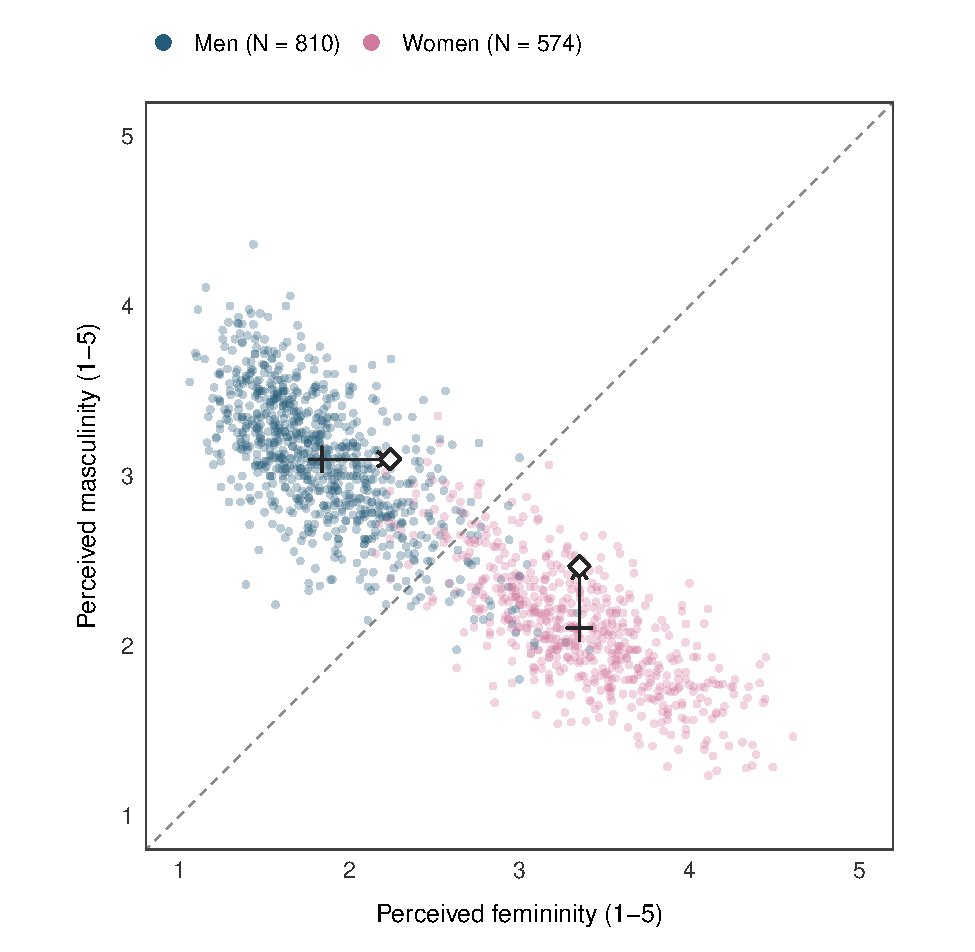
\includegraphics[width=0.78\linewidth]{figures/cue_support.pdf}
\caption{Perceived femininity and masculinity by candidate gender in a combined panel. Blue points show mean ratings for 810 men and pink points show mean ratings for 574 women. Ratings were elicited relative to others of the same age and gender. Crosses mark gender-group average ratings. The dashed diagonal marks equal raw ratings on the 1--5 scales. The gender-atypical contrast is standardized within gender using \autoref{eq:axes}.}
\label{fig:cue-support}
\end{figure}

Because the ratings are gender-referenced, $A=0$ denotes an average relative contrast within the candidate's gender category. This reference point is determined by the gender-specific centering and scaling in \autoref{eq:axes}, whereas the diagonal in Figure~\ref{fig:cue-support} compares the two raw ratings. Zero on the index does not mark a boundary at which observers become uncertain about gender. The index thus measures one aspect of perceived appearance rather than gender identity or categorization difficulty.\footnote{We also estimate balance between the raw ratings, controlling for their mean intensity. \autoref{sec:oa-balance} of the Online Appendix provides this alternative measure's definition and estimates.}

Because the contrast locates candidates within their gender category, Table~\ref{tab:summary} reports the outcome, appearance measures, and covariates separately for men and women in the sample that we exploit below. This organization shows the variation within each category on which the subsequent comparison of electoral inequality rests.

\begin{table}[!htbp]
\centering\small
\caption{Summary statistics by candidate gender}
\label{tab:summary}
\begin{tabular}{@{}lrrc@{\hspace{1.5em}}rrc@{}}
\toprule
 & \multicolumn{3}{c}{Men ($N=810$)} & \multicolumn{3}{c}{Women ($N=574$)} \\
\cmidrule(lr){2-4}\cmidrule(l){5-7}
Variable & Mean & SD & Min.--Max. & Mean & SD & Min.--Max. \\
\midrule
Personal votes & 88.93 & 267.74 & $1$--$4,653$ & 95.22 & 224.34 & $1$--$3,642$ \\
Gender-atypical cue contrast ($A$) & 0.00 & 1.00 & $-2.33$--$3.70$ & 0.00 & 1.00 & $-2.49$--$2.78$ \\
Femininity rating & 1.84 & 0.40 & $1.06$--$3.41$ & 3.35 & 0.47 & $2.16$--$4.61$ \\
Masculinity rating & 3.10 & 0.40 & $1.80$--$4.36$ & 2.11 & 0.36 & $1.24$--$3.35$ \\
Attractiveness rating & 2.76 & 0.45 & $1.44$--$4.02$ & 3.03 & 0.50 & $1.32$--$4.35$ \\
Candidate age (years) & 46.20 & 10.62 & $18$--$63$ & 45.13 & 10.30 & $20$--$63$ \\
\bottomrule
\end{tabular}
\par\smallskip
\begin{minipage}{\linewidth}\footnotesize
$N=1,384$ candidates in 221 municipalities and 10 parties. Summary statistics include means, standard deviations (SD), and observed ranges (Min.--Max.). Appearance measures are candidate averages of 1--5 ratings. Appearance judgments are referenced to people of the same gender and age, so their means do not measure absolute differences between men and women. Within-gender standardization gives $A$ a mean of zero and a standard deviation of one in each category. Candidate age refers to the 2017 election. Personal votes have a median of 37.50 among men (first--third quartiles, 18.00--74.00) and 44.00 among women (19.00--97.75).
\end{minipage}
\end{table}

\section{Empirical strategy}
\label{sec:strategy}
\subsection{An observational natural experiment}
\label{sec:natural-experiment}
We treat naturally arising gendered appearance as an observational natural experiment under the framework for an observational subtype defined by \textcite[118--119]{Titiunik2021}. Researchers neither designed nor implemented the appearance-generating process, and its full allocation probabilities are unknown and unrecoverable. The remaining assignment premise is that this process contains a probabilistic component outside candidates' precise control. Candidates are the units, and their continuous gender-atypical cue contrast describes the appearance condition. \autoref{sec:oa-natural-experiment} maps the application to these three defining conditions.

The external component in this application is naturally arising variation in inherited facial morphology and development. Genetic contributions to normal facial morphology are documented by \textcite{LiuEtAl2012}. We assume that an uncontrollable part of this variation contributes to the balance of gendered cues visible in campaign portraits, leaving candidates with more than one possible appearance condition \emph{ex ante}. Grooming, expression, and portrait selection can shape the visible cues while remaining subject to features candidates cannot choose precisely. Under this assignment premise, external chance can coexist with systematic presentation choices \parencite[118--119]{Titiunik2021}.

The Finnish municipal setting provides substantive grounds for expecting naturally arising differences to remain visible in electoral competition. Parties assemble extensive lists and actively recruit ordinary residents, including people who are not pursuing professional political careers \parencite[628]{Bahamonde2024}. An emphasis on functionality and frugality is reflected in portraits showing everyday clothing alongside formal attire. Campaign communication prominently relies on headshots in posters and newspaper advertisements, with limited individual television and radio campaigning \parencite[628--629]{Bahamonde2024} \parencite[80,83]{BerggrenEtAl2017}. These practices connect a broad candidate pool to routine representations of appearance, supporting the plausibility of the assignment premise within the population of candidates.

We exploit this observational natural experiment to characterize electoral inequality conditional on candidate attributes and electoral context. The classification concerns the origin of appearance variation, while statistical identification comes from comparisons after accounting for municipality, party, age, and attractiveness. We estimate conditional associations because the external assignment premise alone does not establish exchangeability of candidates with different appearance profiles \parencite[119,122--124]{Titiunik2021}.

\subsection{Conditional vote-count specification}
\label{sec:vote-model}
The outcome \texttt{Votes}$_i$ is the number of personal votes received by candidate $i$. Finnish municipal elections use open-list proportional representation. Each voter selects an individual candidate, and the vote also contributes to the candidate's electoral list. Pooled list votes determine the allocation of seats, while personal votes determine candidates' positions within the list \parencite[604,626]{HolliWass2010}. These rules make personal support important for competition among candidates on the same list and for access to representation \parencite[13,16]{SoderlundVonSchoultz2024}. This individual choice also makes the setting relevant to appearance-based evaluation. As \textcite[566]{Lawson2010a} argue, ``Looks should matter more when elections are candidate centered, not party centered''. Personal-vote counts allow us to examine how support is distributed across appearance profiles within this competition, following appearance research using actual election returns \parencite{Efran1974,Bahamonde2024}.

We exploit the original dataset to estimate the expected number of votes conditional on candidate appearance and electoral context. Following \textcite{Bahamonde2024}, we use Poisson pseudo-maximum likelihood (PPML) to estimate the conditional expected vote count. The Poisson specification relates that expectation to the gender-atypical index, while municipality fixed effects account for differences in the scale and shared context of local elections. Party fixed effects account for differences in support across parties. Age and attractiveness enter as candidate controls, and an interaction allows the association between atypicality and votes to differ between men and women.

\begin{equation}
\begin{aligned}
 \mu_i &= \mathrm{E}[\texttt{Votes}_i\mid
 \texttt{Atypicality}_i,\texttt{Woman}_i,\mathbf{X}_i,c(i),p(i)],
 \\[-0.1em]
 \log\mu_i &= \alpha_{c(i)}+\lambda_{p(i)}+\beta_1\texttt{Woman}_i
 +\beta_2\texttt{Atypicality}_i
 +\beta_3(\texttt{Woman}_i\times\texttt{Atypicality}_i)
 \\[-0.1em]
 &\quad+\beta_4\texttt{Age}_i+\beta_5\texttt{Attractiveness}_i.
\end{aligned}
\label{eq:model}
\end{equation}
With \texttt{Atypicality} given by $A$ in \autoref{eq:axes} and \texttt{Woman} indicating a female candidate, the index's association with log expected votes is $\beta_2$ among men and $\beta_2+\beta_3$ among women. The log link yields positive expected vote counts and expresses the appearance association proportionally, allowing percentage differences in support to be compared across municipalities of different sizes. Estimation uses the observed vote counts in their original units.

Statistical identification of the model coefficients relies on variation in appearance and votes after accounting for municipality and party differences, mean-centered age, and measured attractiveness. These adjustments compare candidates facing shared electoral settings and differing in observed appearance. The resulting coefficients describe appearance-associated differences in expected support conditional on those attributes.\footnote{We also adjust for joint cue level, separating the combined rating levels from their contrast in Online Appendix Figures~\ref{fig:oa-joint-votes} and~\ref{fig:oa-joint-share}. Quadratic terms allow the appearance association to change across index values and depend on how the cues combine. Table~\ref{tab:oa-quadratic} reports the coefficients, Table~\ref{tab:oa-nonlinear-tests} their joint tests, and Figure~\ref{fig:oa-surface} the fitted surface.}

The Poisson specification targets this conditional mean without requiring the outcome's entire distribution to be Poisson when the mean is correctly specified \parencite{SantosSilva2006}. The conditional variance may therefore differ from the mean. We also allow outcomes to be dependent among candidates in the same municipality, using municipality-clustered sandwich standard errors with a finite-sample correction and $t_{G-1}$ intervals, where $G$ is the number of municipalities. These intervals condition on the candidate mean ratings used to construct the contrast and do not propagate uncertainty in those estimated means. \autoref{sec:oa-diagnostics} of the Online Appendix reports dispersion and sample diagnostics.

Figure~\ref{fig:predicted-votes} translates the fitted associations into expected personal votes, making the distribution of support across appearance profiles visible within each gender category.\footnote{At each index value $a$, we predict votes for each candidate while retaining observed age, attractiveness, party, and municipality. Averaging over the $n_g$ candidates in gender group $g$ gives \begin{equation}\overline{\mu}_g(a)=\frac{1}{n_g}\sum_{i:g(i)=g}\widehat{\mu}_i(a).\label{eq:predictions}\end{equation} The curves describe expected personal votes rather than seat-winning probabilities.} Comparing points along each curve therefore holds the group's other observed characteristics constant.\footnote{Online Appendix \autoref{eq:share-predictions} defines average municipal vote shares, and Figure~\ref{fig:predicted-share} expresses the same fitted model on that scale.}

\begin{figure}[!htbp]
\centering
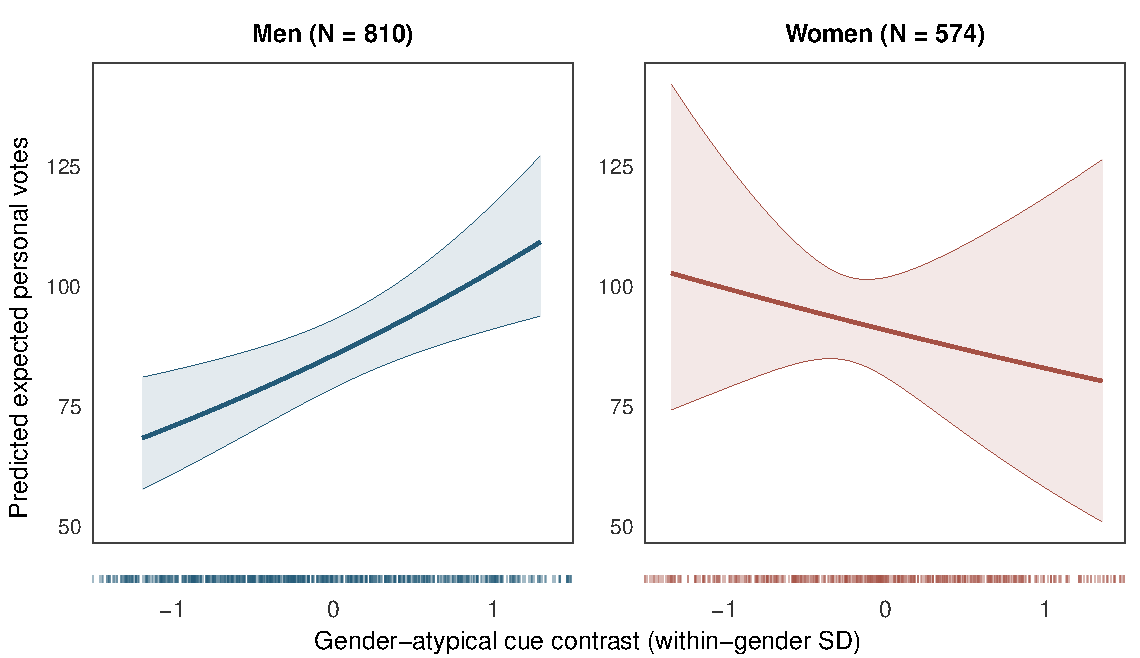
\includegraphics[width=0.92\linewidth]{figures/predicted_votes.pdf}
\caption{Predicted expected personal votes in the observational natural experiment, with baseline controls. Curves vary the atypical cue contrast over the within-gender 10th--90th percentile range and average over observed candidate characteristics, parties, and municipalities. Shading gives municipality-clustered 95\% confidence intervals for the conditional mean. Rug strips beneath each panel show observed candidates within the displayed cue range. Panel headings report the full gender-group sample sizes.}
\label{fig:predicted-votes}
\end{figure}

\section{Results}
\label{sec:results}
Figure~\ref{fig:predicted-votes} presents the main results as differences in expected personal support across appearance profiles.\footnote{Table~\ref{tab:oa-baseline-regression} in the Online Appendix presents the corresponding Poisson regression table, reporting coefficients and municipality-clustered standard errors for the baseline model underlying Figure~\ref{fig:predicted-votes}.} Table~\ref{tab:main} quantifies those differences for a one-SD increase in the gender-atypical contrast. The estimated differences in expected votes are 20.7\% (95\% CI 8.0\% to 35.0\%) for men and -8.8\% (95\% CI -31.1\% to 20.8\%) for women. Within male candidacies, expected personal votes favor more gender-atypical cue profiles. The female association is inconclusive.\footnote{The direct test of the difference between the gender-specific associations gives $p=0.054$.}
\par

\begin{table}[!htbp]
\centering
\small
\caption{Gender-atypical appearance and expected personal votes with baseline controls}
\label{tab:main}
\begin{tabular}{lcc}
\toprule
Cue & Men (\%) & Women (\%) \\
\midrule
Gender-atypical contrast ($A$) & 20.7 [8.0, 35.0] & -8.8 [-31.1, 20.8] \\
\bottomrule
\end{tabular}
\begin{minipage}{\linewidth}\footnotesize
Entries are percentage differences in expected votes for a one-SD increase in the atypical cue contrast, with municipality-clustered 95\% confidence intervals in brackets. The model includes 1384 candidates in 221 municipalities, with municipality and party fixed effects, age, and attractiveness.
\end{minipage}
\end{table}

These results bring the inequality question into focus. Among men, the baseline model associates greater expected personal votes with more feminine-relative-to-masculine profiles, locating appearance-associated inequality within the gender category. This within-male advantage runs against the conformity expectation that departure from masculine appearance norms reduces personal support. This is consequential for inequality against women if men have more room to convert departure into a valued leadership profile, while women face tighter constraints on combining authority with expected warmth.

The cooperative-leadership account explains why such unequal latitude could arise. More feminine liberal men were judged warmer in \textcite{CarpinellaJohnson2013b}, and feminine-looking leaders gained value in peacekeeping scenarios in \textcite{SpisakWarriors2012}. If voters value cooperation, feminine cues can consequently offer men a route to greater support despite departing from masculine appearance expectations. This route has an inequality implication because communality can be rewarded as an additional quality in men while remaining an expectation placed on women. The male communality bonus in \textcite{Hentschel2018} provides a parallel in leadership evaluations, while the competing prescriptions identified by \textcite{Eagly2002} and \textcite{RudmanGlick2001} explain why women may have less latitude to gain from the opposite departure. The proposed source of inequality is therefore the gendered standard governing which departures become assets.

This interpretation concerns relative appearance within each gender category. \textcite{Park2023} report a positive association between perceived masculinity and US vote share, whereas we compare the balance of femininity and masculinity relative to same-gender peers.\footnote{Our index can increase through higher femininity, lower masculinity, or both. \textcite{Park2023} evaluate whole campaign photographs and enter the cues separately. Their masculinity coefficient and our within-gender cue contrast therefore describe different comparisons.} The two studies ask how different appearance profiles attract support, and both make political context relevant to that question. We therefore turn to party-specific comparisons to examine where departure is associated with advantage and where it is associated with disadvantage.

\subsection{Party-specific associations}
The contextual expectation implies that inequality within a gender category may take a different direction or magnitude across political settings. We exploit the dataset's party information to examine this implication, allowing cue slopes and gender intercepts to vary by candidate party while retaining the baseline controls. Let $\log\mu_i^{\mathrm{baseline}}$ denote the linear predictor in \autoref{eq:model}. The secondary specification is
\begin{equation}
\begin{aligned}
 \log\mu_i^{\mathrm{party}} &= \log\mu_i^{\mathrm{baseline}}
 +\sum_{p\ne p_0}\mathbf{1}(\texttt{Party}_i=p)
 \left[\delta_p\texttt{Woman}_i+\kappa_p\texttt{Atypicality}_i\right.
 \\[-0.1em]
 &\qquad\left.+\tau_p(\texttt{Woman}_i\times\texttt{Atypicality}_i)\right],
\end{aligned}
\label{eq:party-model}
\end{equation}
Relative to reference party $p_0$, the additional terms allow the atypicality association to vary across parties and by gender within each party. Re-estimating all coefficients retains the baseline log link and expresses these associations as proportional differences in expected votes. We keep the within-gender atypicality scale defined in \autoref{eq:axes}, so each party comparison uses the same unit of departure. The model includes 1380 candidates in 8 parties and 221 municipalities.\footnote{We restrict party-specific comparisons to parties with at least 5 candidates in each gender category. This excludes PIR (2 men, 1 woman) and SKP (1 man, 0 women), totaling 4 candidates. They remain in the primary analysis. Online Appendix Table~\ref{tab:oa-party} reports the party-specific contrasts and candidate and municipality counts. Candidate party identifies the political setting, while voters' individual ideologies are unobserved.}

Figure~\ref{fig:party-votes} disaggregates the appearance-associated inequality summarized in Figure~\ref{fig:predicted-votes}.\footnote{Predictions average over observed candidate characteristics and municipalities within each party and gender. Rug strips show observed cue profiles. Confidence bands are omitted to emphasize substantive point-estimate patterns. Municipality-clustered intervals and joint heterogeneity tests appear in \autoref{sec:oa-party} of the Online Appendix. Panels use separate vertical scales, and their levels reflect group composition. Table~\ref{tab:oa-party} provides the proportional contrasts for comparing slopes.} Within the National Coalition Party, the fitted associations favor a more feminine-relative-to-masculine profile in both gender groups. The one-standard-deviation atypicality contrasts are 22.1\% among men and -38.0\% among women. The opposing index signs reflect departure from male appearance norms and conformity to female appearance norms.

Among women, the fitted association favors more masculine-relative-to-feminine profiles in the Centre Party and more feminine-relative-to-masculine profiles in the Green League. The one-standard-deviation atypicality contrasts are 63.0\% in the Centre Party and -46.7\% in the Green League. These opposing point estimates locate potential appearance advantages within gender and party contexts. These differences matter for the argument about inequality against women. The negative female point estimates locate settings in which departure from feminine appearance expectations is associated with less support, while the positive Centre Party estimate suggests a setting in which the same departure could become an asset. Political context may therefore change how restrictive the competing demands for warmth and authority are for women.

This variation connects the findings to the candidate gender-by-party differences reported by \textcite{Carpinella2016}. In their actual-election models, less masculine Republican men and more feminine Republican women were more likely to win. That pattern makes the gendered standards relevant to appearance rewards visible, since a feminine profile departs from male expectations while conforming to female expectations. Their vote-margin analysis yielded a different pattern, which makes the electoral outcome being studied part of the comparison. We exploit personal-vote counts to examine how these gendered rewards enter the allocation of support within Finnish party lists.

The party comparisons also clarify why the leadership interpretation must include the audience. \textcite{LaustsenPetersen2016} show that liberal and conservative audiences place different electoral value on facial dominance. If party audiences likewise differ in the weight they place on warmth and authority, a feminine male profile or a masculine female profile could attract different rewards across settings. The substantive implication is that women's opportunities to benefit from departure may depend on which political audience evaluates them.

Of the 16 party--gender contrasts, 9 are not statistically significant at the 5\% level. We therefore use these point-estimate patterns to develop the contextual interpretation of inequality. The corresponding sensitivity checks show how adjustment for prior office and unusually high vote counts changes the party comparisons.\footnote{Online Appendix Table~\ref{tab:oa-party-sensitivity} reports these comparisons. The National Coalition male contrast changes from 22.1\% to -4.9\% with prior-office controls. The Green male contrast changes from 27.9\% to -27.7\% after excluding the highest-vote 1\% of candidates. Within Social Democratic male candidacies, the fitted one-SD contrast in expected personal votes changes from 213.5\% to 28.9\% after prior-office adjustment.}

\begin{figure}[!htbp]
\centering
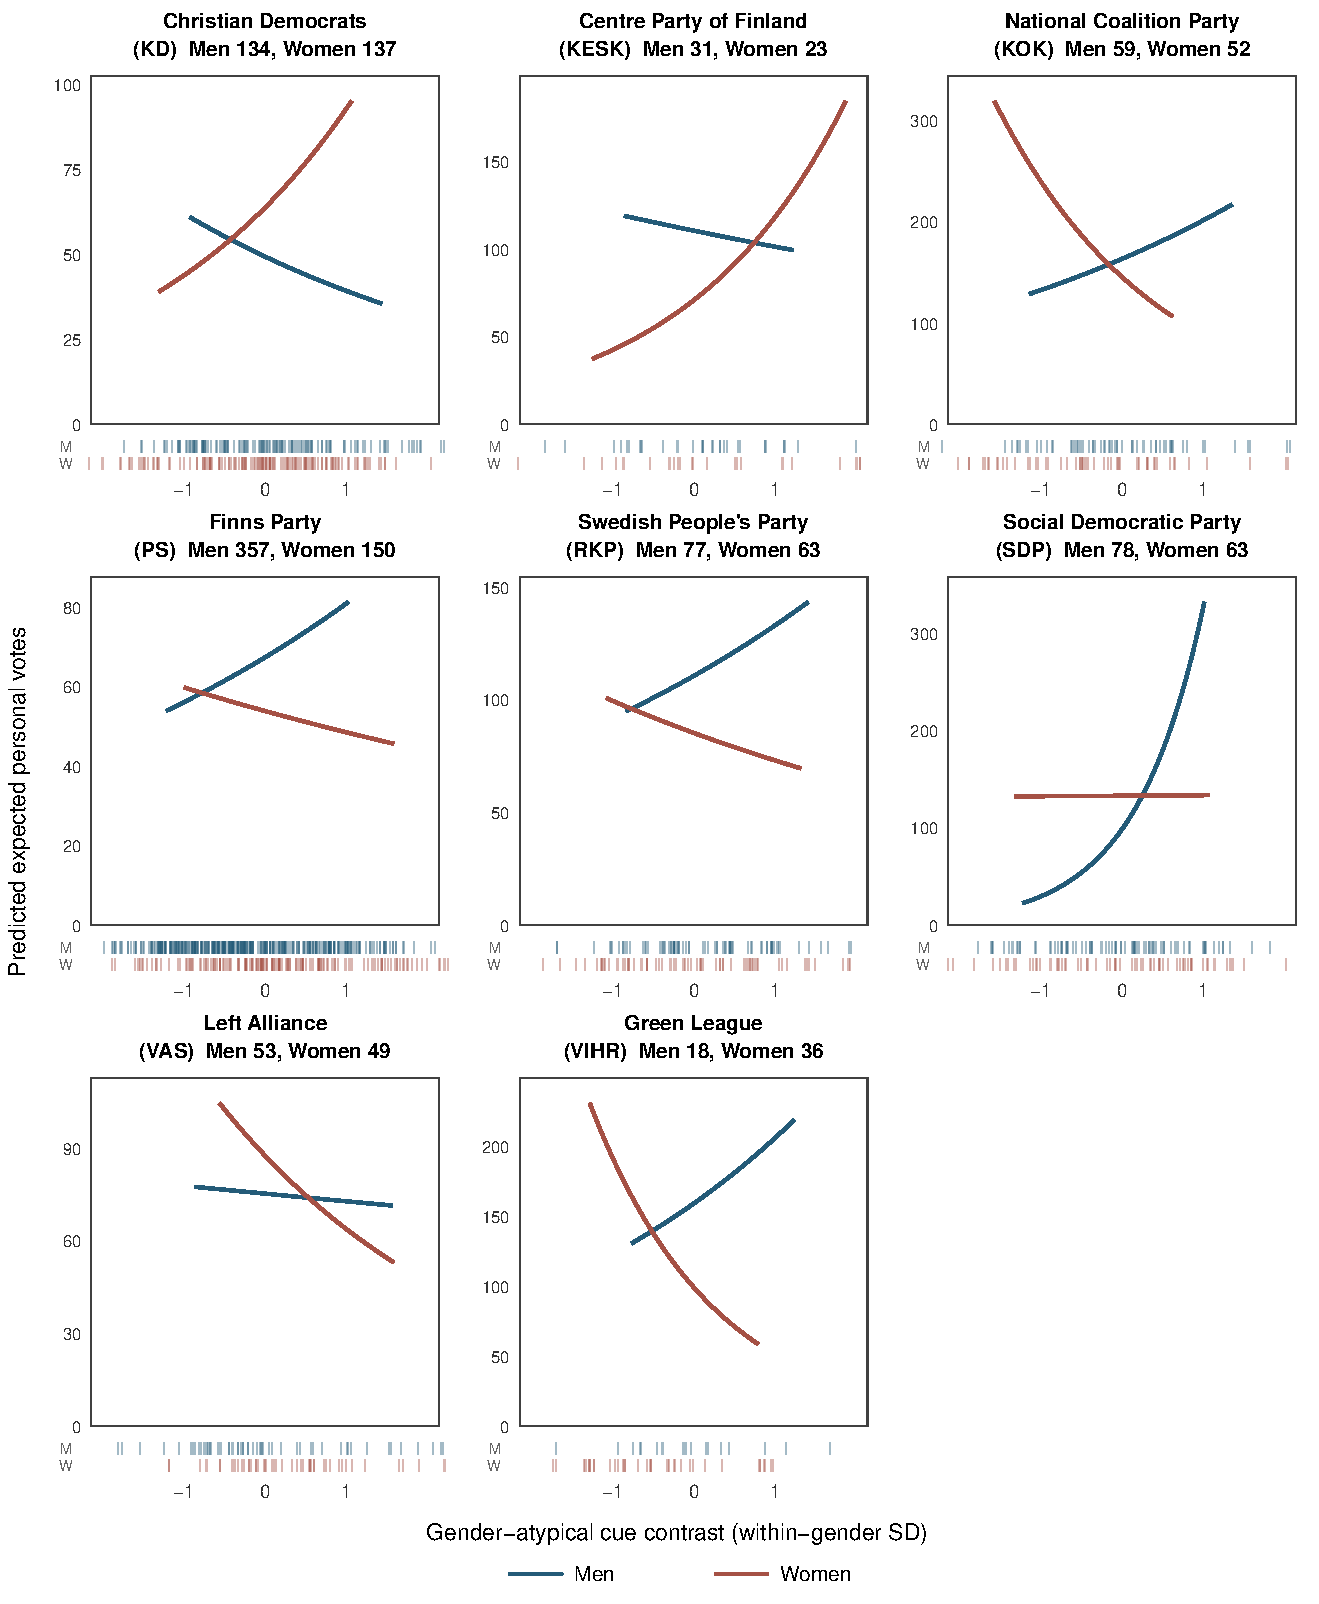
\includegraphics[width=\linewidth]{figures/party_predicted_votes.pdf}
\caption{Predicted expected personal votes by party and gender, with baseline controls. Curves vary the cue contrast over each party--gender group's 10th--90th percentile range and average over that group's observed candidate contexts. Each solid curve shows the continuous fitted predictions throughout this range. Confidence bands are omitted. 9 of the 16 party--gender contrasts are not statistically significant at the 5\% level. Online Appendix Table~\ref{tab:oa-party} reports intervals for the corresponding one-SD contrasts. Rug strips show observed candidates within the displayed cue range, with men (M) above women (W). Panel headings report full group sample sizes. Vertical scales differ between panels.}
\label{fig:party-votes}
\end{figure}


\subsection{Distinguishing gendered appearance from attractiveness}
\label{sec:attractiveness}
Does the appearance-associated inequality simply reflect differences in attractiveness? This is a consequential alternative because attractive candidates can receive more votes \parencite{BerggrenEtAl2010,Bahamonde2024}. If the gender-atypical index merely captured attractiveness, it would add little to the explanation of unequal support. Our original dataset allows us to examine that possibility directly because attractiveness, masculinity, and femininity were rated separately. We exploit these measurements to compare how the scores relate to one another and whether accounting for attractiveness explains the appearance-associated differences in votes.

Figure~\ref{fig:attractiveness-pairs} pairs each candidate's gender cue balance with that candidate's attractiveness rating, separately for men and women. This comparison shows whether relatively feminine appearance is associated with greater measured attractiveness among candidates of the same gender. We use the signed cue balance $B=A$ among men and $B=-A$ among women. This orientation places relatively masculine profiles at lower values and relatively feminine profiles at higher values in both groups, with zero corresponding to each group's average balance.

Among men, the two measurements have little linear or rank-order relationship. The Pearson correlation is 0.064, and the Spearman correlation is 0.056. A more feminine appearance relative to masculine appearance therefore does not simply pick out the men rated as more attractive. Among women, the corresponding correlations are 0.764 and 0.744. Women rated as more feminine relative to masculine are also commonly rated as more attractive. This overlap recalls \textcite[42--43]{Sigelman1987a}, whose female-candidate experiment linked perceived femininity to greater niceness and lower dynamism, with a favorable net association with support.

\begin{figure}[!htbp]
\centering
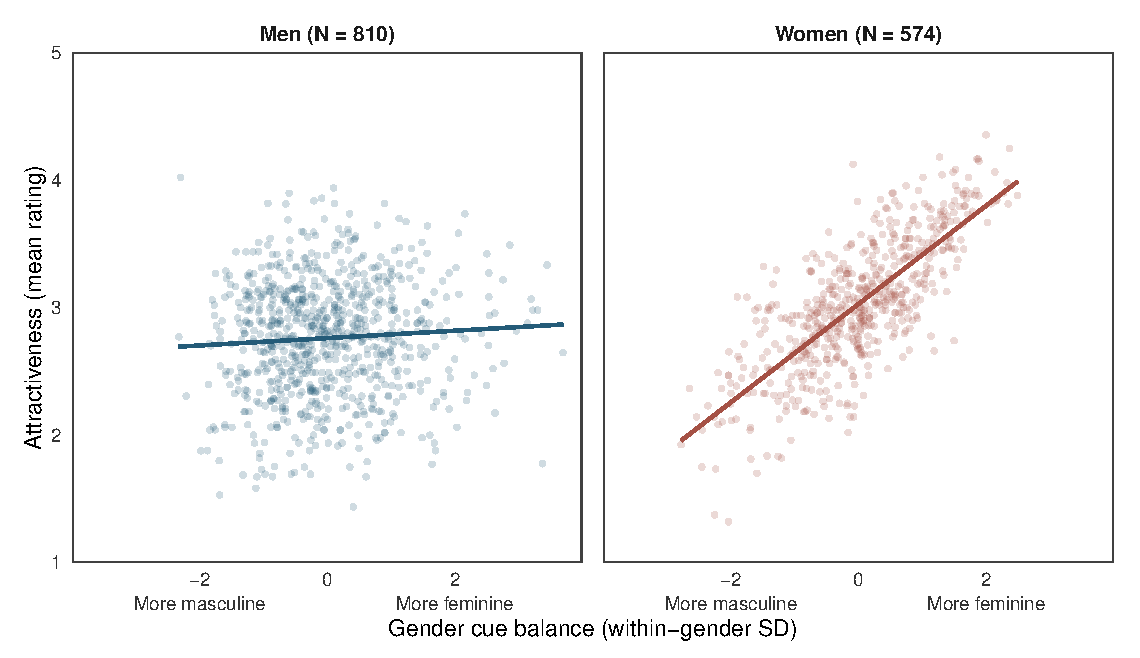
\includegraphics[width=\linewidth]{figures/attractiveness_cue_pairs.pdf}
\caption{Gender cue balance and attractiveness by recorded gender. Each point pairs one candidate's signed cue balance $B$ with that candidate's mean attractiveness rating. Lines summarize the paired relationships using descriptive least-squares fits. $B$ increases with femininity relative to masculinity within either gender. $B=A$ for men and $B=-A$ for women. Headings report group sample sizes. Attractiveness uses the 1--5 rating scale.}
\label{fig:attractiveness-pairs}
\end{figure}

The next comparison asks whether attractiveness adjustment accounts for the observed difference in electoral support. Table~\ref{tab:attractiveness-adjustment} compares three Poisson specifications on the same 1384 candidates. The first omits attractiveness, the baseline includes it as a linear control, and the third allows the attractiveness association to vary by gender and take a nonlinear form. The flexible specification uses natural cubic splines with 3 degrees of freedom, interacted with gender. All three retain the same age, party, and municipality controls and the same gender-atypical index. This comparison changes the treatment of measured attractiveness while holding the other parts of the comparison constant.

\begin{table}[!htbp]
\centering\small
\caption{Atypicality contrasts under alternative attractiveness adjustments}
\label{tab:attractiveness-adjustment}
\begin{tabular}{p{0.40\linewidth}rcc}
\toprule
Attractiveness adjustment & $N$ & Men (\%) & Women (\%) \\
\midrule
Attractiveness omitted & 1384 & 18.7 [3.7, 35.9] & -32.6 [-44.5, -18.2] \\
Baseline linear attractiveness & 1384 & 20.7 [8.0, 35.0] & -8.8 [-31.1, 20.8] \\
Gender-specific attractiveness spline & 1384 & 21.0 [8.1, 35.5] & -16.4 [-34.6, 7.0] \\
\bottomrule
\end{tabular}
\begin{minipage}{\linewidth}\footnotesize
Entries are percentage differences in expected personal votes for a one-SD increase in $A$, with municipality-clustered 95\% intervals in brackets. All specifications use the same 1384 candidates and retain all other baseline controls. The flexible adjustment uses gender-specific natural cubic splines for attractiveness.
\end{minipage}
\end{table}

Among men, the one-standard-deviation cue contrasts are 18.7\% without attractiveness adjustment, 20.7\% with the baseline adjustment, and 21.0\% under gender-specific nonlinear attractiveness adjustment. Flexible attractiveness adjustment supports an appearance-associated advantage for more gender-atypical male profiles. This pattern is consistent with a cue association distinct from measured attractiveness.

Among women, the corresponding contrasts are -32.6\% without attractiveness adjustment and -8.8\% with the baseline adjustment. The flexible estimate is -16.4\% (95\% CI -34.6\% to 7.0\%). The adjusted female association is inconclusive.

The attractiveness comparisons help distinguish the proposed source of inequality from a general beauty premium. Among men, cue balance has little relationship with measured attractiveness, and the appearance-associated advantage persists after flexible attractiveness adjustment. The male reward for departure therefore extends beyond the beauty ratings in the dataset. Among women, femininity and attractiveness are more closely aligned, connecting the expectation of feminine appearance to another valued electoral attribute. This overlap makes those competing standards relevant to the interpretation, since the appearance theorized to convey feminine warmth is also commonly rated as attractive. The model comparisons consequently sharpen the argument about unequal opportunities to benefit from appearance.

\section{Discussion}
\label{sec:discussion}
Does departure from gender stereotypes carry an electoral penalty? Exploiting an original dataset of separately rated appearance cues and linked electoral returns, we find that departure can be associated with electoral advantage among men, while the pooled female estimate is inconclusive. The inequality question is consequently about who has room to turn gender-atypical appearance into a resource. The male association directs attention to the possibility that men can benefit from feminine cues, while women face competing expectations of feminine warmth and leadership authority. Party comparisons develop this interpretation by locating settings with different appearance rewards.

This interpretation connects inequalities within gender categories to the competing standards women face. \textcite{Monk2022}'s perspective reveals why category membership alone cannot describe the distribution of rewards among candidates. Combining that perspective with gendered leadership expectations asks whether some departures become assets for men while others expose women to conflicting standards \parencite{Eagly2002,RudmanGlick2001}. Warmth provides a possible route to such unequal rewards because a quality expected of women can become an additional leadership asset for men \parencite{CarpinellaJohnson2013b,Hentschel2018}. The party patterns make the political audience part of this account, suggesting that women's latitude to depart may depend on which leadership qualities are valued in their setting.

These appearance rewards matter for representation because personal votes determine candidates' positions within electoral lists \parencite{HolliWass2010,SoderlundVonSchoultz2024}. When a profile receives greater support, candidates who display it gain an advantage in that competition. Gender inequality can therefore operate through the standards governing which appearances become electoral assets, as well as through differences in support between men and women overall. Focusing on these standards links within-category comparisons to the opportunities women face when seeking political office.

The study's observational design sets the scope of this interpretation. The natural-experiment classification rests on an assumed external probabilistic component in appearance, whose assignment law is unrecoverable \parencite[118--119]{Titiunik2021}. Grooming and portrait selection shape the observed cues, while entry into candidacy, recognition, and campaign resources can relate appearance to electoral prospects. The fixed effects and controls identify conditional associations rather than causal effects of changing appearance. Attractiveness adjustment likewise describes an association conditional on measured beauty, leaving the underlying perceptual pathway for further investigation.

The scope of the evidence also depends on the sample and measurements. Estimates vary with prior-office adjustment and the treatment of unusually high-vote candidates.\footnote{Online Appendix Table~\ref{tab:oa-sensitivity} compares municipality-by-party fixed effects, separate-gender specifications, and upper-tail vote exclusions. Figures~\ref{fig:oa-votes} and~\ref{fig:oa-share} compare predictions with and without incumbency and parliamentary-office controls. Table~\ref{tab:oa-party-sensitivity} reports the corresponding party comparisons.} The post-election ratings reflect Finnish-speaking adults in the survey's age range, while voters' own trait inferences and ideology are unobserved. The vote-model intervals condition on candidates' mean ratings. These features make direct tests of voter perceptions and replication across electorates the next steps in assessing unequal latitude to depart from gender expectations.

Future research can test that argument by independently varying femininity, masculinity, and attractiveness in matched candidate portraits. Measuring warmth and competence would then show which impressions connect appearance to support, while cooperative and competitive leadership tasks would establish when each impression matters. Varying party labels and measuring voter ideology would further identify the audiences under which women face tighter or looser constraints on appearance. Repeated portraits and information on prospective candidates could establish how presentation and recruitment shape the appearance profiles that reach elections. Together, these designs would clarify when departure becomes an asset for men and whether women face penalties or fewer opportunities to gain the same advantage.

% AMBIGUITY_MAIN_END
\newpage

\FloatBarrier
\printbibliography[title={References}]

\newpage


\FloatBarrier
\appendix
\section*{Online Appendix}
\addcontentsline{toc}{section}{Online Appendix}
\setcounter{figure}{0}
\setcounter{table}{0}
\setcounter{equation}{0}
\renewcommand{\thefigure}{OA~\arabic{figure}}
\renewcommand{\thetable}{OA~\arabic{table}}
\renewcommand{\theequation}{OA~\arabic{equation}}
\renewcommand{\theHfigure}{oa.\arabic{figure}}
\renewcommand{\theHtable}{oa.\arabic{table}}
\renewcommand{\theHequation}{oa.\arabic{equation}}
\renewcommand{\thesection}{OA~\arabic{section}}
\setcounter{section}{0}

\section{A natural experiment as a subtype of observational study}
\label{sec:oa-natural-experiment}

\textcite[118--119]{Titiunik2021} defines a natural experiment as a special kind of observational study through three conditions on the assignment mechanism. Researchers neither design nor implement assignment, its full probability law is unknown and unknowable to them, and an external factor outside the units' direct control makes assignment probabilistic. Her Definition NE denotes these conditions by $\widetilde D$, $\widetilde K$, and $\widetilde P$. We apply each condition to the process generating candidates' gendered appearance. Candidates are the units, their appearance condition is summarized by the continuous within-gender contrast $A_i$ in \autoref{eq:axes}, and personal votes are the outcome. Let $\mathbf A_g$ collect the appearance conditions of the candidates in gender category $g$ represented in the dataset, and let $Q_g$ denote their joint assignment law. Following Definition NE, this law is conditional on predetermined characteristics and the potential-outcome schedule, with the conditioning suppressed below.

\subsection{Assignment outside the researchers' control}

Condition $\widetilde D$ requires that researchers neither design nor implement the assignment mechanism. In our study, the facial characteristics visible in campaign portraits arose before and independently of the research project. We observed existing candidates and their portraits without allocating facial features or directing how candidates presented themselves in the election. The process assigning gendered appearance therefore operated outside the researchers' control, satisfying the first condition.

\subsection{An unknown and unrecoverable assignment mechanism}

Condition $\widetilde K$ requires that the assignment mechanism be unknown and unknowable to the researchers. In this application, $Q_g$ is the full law governing alternative allocations of appearance conditions across candidates. No recoverable allocation protocol supplies the probabilities that particular candidates would have received alternative facial profiles. The portraits and electoral records contain the realized appearance conditions, while the full probabilities generating those conditions remain inaccessible. Knowing the formula for the index or the distribution of observed scores does not recover $Q_g$. The appearance-assignment mechanism is therefore unknown and unrecoverable for this design, which places the study within the observational category in the framework.

\subsection{A probabilistic component arising from an external factor}

Condition $\widetilde P$ requires probabilistic assignment arising from an external event or intervention outside the units' direct control. Our external factor is naturally arising variation in inherited facial morphology and development. Genetic contributions to normal facial morphology are documented by \textcite{LiuEtAl2012}. We assume that an uncontrollable component of this variation contributes to the gendered cue contrast among the candidates represented in the dataset. Candidates can choose grooming, facial expression, and portraits while lacking precise control over all the facial features those portraits display. Such presentation choices can coexist with the external chance component contemplated by the definition \parencite[118--119]{Titiunik2021}.

To express this mapping, let $E_i$ denote the external component and $L_i$ denote presentation choices, with $A_i=\psi_g(E_i,L_i)$ summarizing their contribution to gendered appearance. The assignment premise is that variation in $E_i$ leaves more than one possible value of the contrast for candidate $i$. The original binary formulation expresses probabilistic assignment through a positive probability of either condition \parencite[108]{Titiunik2021}. Our continuous counterpart uses disjoint neighborhoods $B_{i0}$ and $B_{i1}$ of possible contrast values. If $Q_{ig}$ denotes candidate $i$'s marginal law under $Q_g$, the premise is
\begin{equation}
 0<Q_{ig}(B_{ik})<1,
 \qquad B_{i0}\cap B_{i1}=\varnothing,
 \qquad k\in\{0,1\}.
\label{eq:ne-probabilistic-support}
\end{equation}
This condition concerns positive probabilities over distinct ranges of appearance, rather than positive probability at each exact real-valued score. It states the probabilistic appearance-assignment assumption underlying our application of $\widetilde P$.

Finnish municipal recruitment and campaign practices provide the setting in which this external variation enters electoral competition. Parties recruit ordinary residents to extensive candidate lists, and headshots feature prominently in campaign communication \parencite[628--629]{Bahamonde2024}. These practices support the premise that naturally arising differences remain visible in the candidate portraits. Under the stated probabilistic-assignment premise, the case satisfies the three conditions together. Appearance is assigned outside the research project, the full allocation probabilities are unrecoverable, and an external component beyond candidates' precise control contributes chance variation to their gendered cue profiles. The study is therefore a natural experiment within this framework for observational studies.

\section{Balance between raw ratings}
\label{sec:oa-balance}
An alternative specification assesses whether balance between the raw femininity and masculinity ratings is associated with electoral support. It replaces the directional contrast of within-gender standardized ratings with raw cue balance and raw cue intensity, defined in \autoref{eq:raw-balance}.
\begin{equation}
\begin{aligned}
 \texttt{RawBalance}_i &= 1-\frac{|F_i-M_i|}{4},\\
 \texttt{RawIntensity}_i &= (F_i+M_i)/2.
\end{aligned}
\label{eq:raw-balance}
\end{equation}
We standardize each index within gender. The balance associations are 39.0\% (95\% CI 17.2\% to 64.8\%) for men and -10.3\% (95\% CI -30.9\% to 16.4\%) for women. This alternative concerns equality of raw ratings, which is distinct from equality relative to gender-specific means and does not establish categorical uncertainty.

\section{Joint cue level as an additional adjustment}
The directional contrast summarizes relative cue balance but omits the combined rating level. Candidates can have the same directional difference while their combined femininity and masculinity rating levels vary. To assess whether this additional variation changes the atypicality association, we define joint cue level as
\begin{equation}
 S_i=\frac{z^F_i+z^M_i}{\operatorname{sd}_g(z^F+z^M)}.
 \label{eq:joint-level}
\end{equation}
As a standardized sum, $S$ can be elevated when either rating exceeds its gender-specific mean, even if the other falls below it. Conditional on a fixed atypicality contrast, an increase in $S$ corresponds to equal increases in both standardized ratings. The adjusted specification includes $S$ and its gender interaction.
\begin{equation}
\begin{aligned}
 \log\mu_i^{\mathrm{joint}}&=\log\mu_i^{\mathrm{baseline}}
 +\rho_1\texttt{JointCueLevel}_i\\
 &\quad+\rho_2(\texttt{Woman}_i\times\texttt{JointCueLevel}_i).
\end{aligned}
\label{eq:joint-model}
\end{equation}
All baseline coefficients are re-estimated. This adjustment relaxes the equal-magnitude, opposite associations assigned to standardized femininity and masculinity by the primary contrast specification. The adjusted atypicality associations are 20.4\% (95\% CI 7.9\% to 34.4\%) for men and -13.5\% (95\% CI -37.7\% to 20.3\%) for women. The joint-level associations are 8.9\% (95\% CI -11.0\% to 33.1\%) and 15.6\% (95\% CI -10.1\% to 48.5\%), respectively. Figures~\ref{fig:oa-joint-votes} and~\ref{fig:oa-joint-share} compare the predictions from both specifications. Table~\ref{tab:oa-sensitivity} reports the corresponding atypicality contrasts. Holding joint cue level constant, the estimated gradient favors more gender-atypical profiles within male candidacies. The separate joint-level associations are inconclusive in both gender groups.

\begin{figure}[!htbp]
\centering
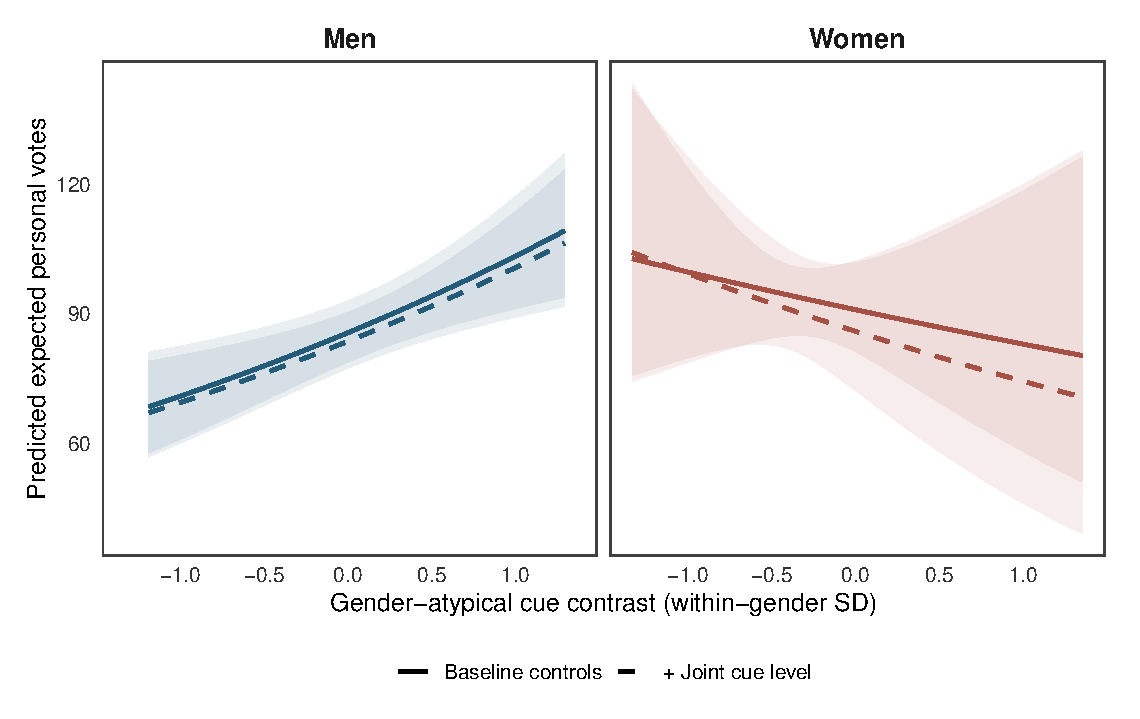
\includegraphics[width=0.92\linewidth]{figures/oa_joint_predicted_votes.pdf}
\caption{Predicted expected personal votes with and without joint cue level. The adjusted curve holds $S=0$. The baseline model does not include $S$. Both specifications average predictions over the same gender-specific observed candidate contexts. Shading denotes municipality-clustered 95\% confidence intervals.}
\label{fig:oa-joint-votes}
\end{figure}

\begin{figure}[!htbp]
\centering
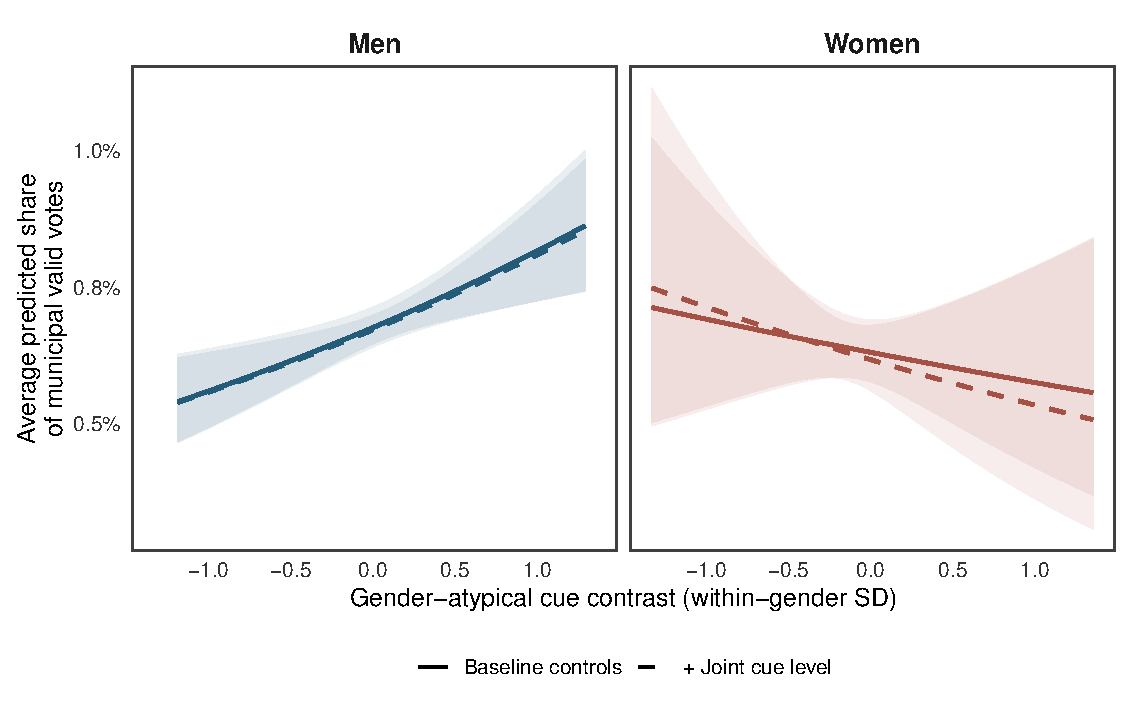
\includegraphics[width=0.92\linewidth]{figures/oa_joint_predicted_vote_probability.pdf}
\caption{Average predicted municipal vote share with and without joint cue level. Predictions and confidence intervals follow Figure~\ref{fig:oa-joint-votes}. Denominators include all valid personal votes in each municipality.}
\label{fig:oa-joint-share}
\end{figure}

\FloatBarrier
\section{Quadratic cue configurations}
The joint-level adjustment permits the directional contrast and combined rating level to vary independently. Its linear predictor nevertheless estimates constant slopes of log expected votes for both cue indices within gender. To allow curvature and an atypicality slope that varies with joint level, the quadratic specification adds squared indices, their product, and gender interactions to \autoref{eq:joint-model}.
\begin{equation}
\begin{aligned}
 \log\mu_i^{\mathrm{quadratic}} &= \log\mu_i^{\mathrm{joint}}
 +\eta_1\texttt{Atypicality}_i^2+\eta_2\texttt{JointCueLevel}_i^2
 \\
 &\quad+\eta_3\texttt{Atypicality}_i\texttt{JointCueLevel}_i \\
 &\quad+\texttt{Woman}_i\left(
 \eta_4\texttt{Atypicality}_i^2+\eta_5\texttt{JointCueLevel}_i^2
 \right)\\
 &\quad+\eta_6\texttt{Woman}_i\texttt{Atypicality}_i\texttt{JointCueLevel}_i.
\end{aligned}
\label{eq:quadratic}
\end{equation}
All coefficients of the joint-level-adjusted linear predictor are re-estimated, so the added terms describe curvature and interaction conditional on the same controls. Table~\ref{tab:oa-quadratic} reports these nonlinear coefficients by gender. A joint Wald test evaluates whether the 6 added terms equal zero. It gives $F=2.50$ with 6 and 220 degrees of freedom ($p=0.023$). Table~\ref{tab:oa-nonlinear-tests} applies the same test after upper-tail exclusions, connecting the assessment of nonlinearity to dependence on high-vote candidates. Figure~\ref{fig:oa-surface} shows the fitted cue surface only where nearby candidate profiles provide empirical support. Figure~\ref{fig:cue-support} shows the underlying raw ratings. The full-sample joint test supports added quadratic or interaction terms. The joint test is inconclusive under both upper-tail exclusions. This omnibus test concerns the added terms jointly across genders.

\begin{table}[!htbp]
\centering
\caption{Quadratic cue coefficients by candidate gender}
\label{tab:oa-quadratic}
\begin{tabular}{llrrr}
\toprule
Gender & Term & Coefficient & Cluster SE & $p$ \\
\midrule
Men & $A^2$ & -0.143 & 0.058 & 0.014 \\
Men & $S^2$ & 0.012 & 0.066 & 0.855 \\
Men & $A S$ & 0.108 & 0.088 & 0.221 \\
Women & $A^2$ & -0.036 & 0.049 & 0.469 \\
Women & $S^2$ & -0.040 & 0.044 & 0.362 \\
Women & $A S$ & -0.196 & 0.103 & 0.059 \\
\bottomrule
\end{tabular}
\begin{minipage}{\linewidth}\footnotesize
Coefficients are on the log conditional-mean scale. Female coefficients combine each nonlinear term with its gender interaction. Standard errors and $p$-values use the full municipality-clustered covariance matrix. The model includes 1384 candidates in 221 municipalities.
\end{minipage}
\end{table}

\begin{table}[!htbp]
\centering
\caption{Joint tests of the quadratic terms}
\label{tab:oa-nonlinear-tests}
\begin{tabular}{lrrrrr}
\toprule
Specification & $N$ & $F$ & $df_1$ & $df_2$ & $p$ \\
\midrule
Quadratic, full sample & 1384 & 2.504 & 6 & 220 & 0.023 \\
Excluding top 1\% of votes & 1370 & 1.654 & 6 & 220 & 0.134 \\
Excluding top 5\% of votes & 1314 & 1.058 & 6 & 220 & 0.389 \\
\bottomrule
\end{tabular}
\begin{minipage}{\linewidth}\footnotesize
Wald $F$ tests use municipality-clustered standard errors and the joint null that all added quadratic terms equal zero. The numerator degrees of freedom equal the number of tested terms. Denominator degrees of freedom equal $G-1$.
\end{minipage}
\end{table}

\begin{figure}[!htbp]
\centering
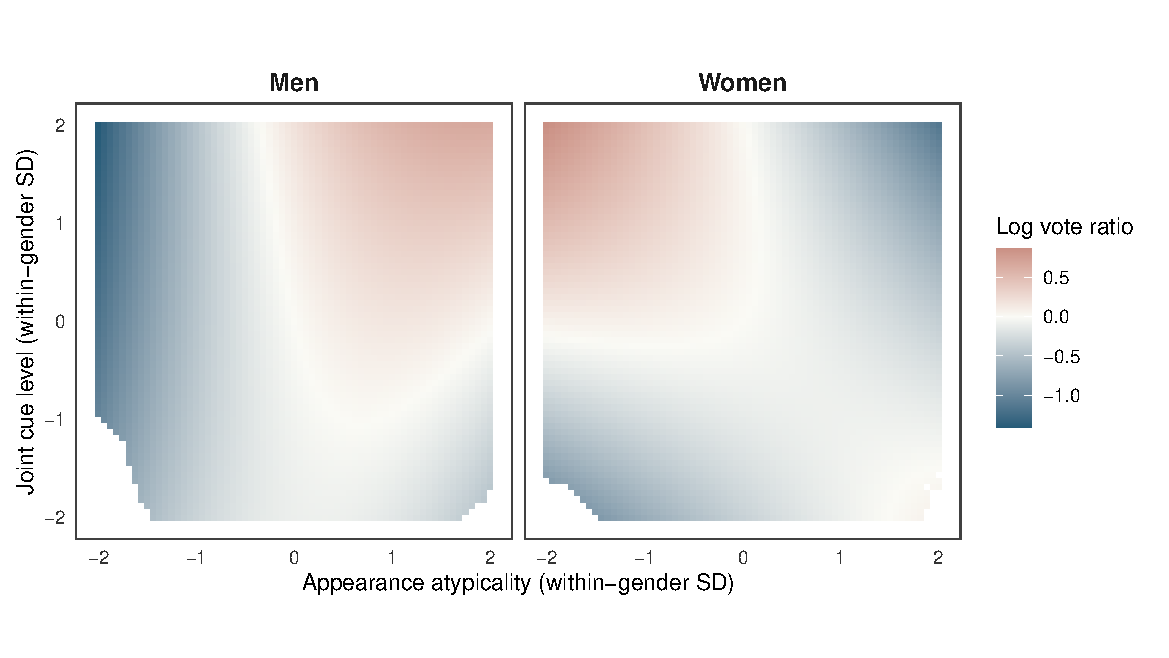
\includegraphics[width=\linewidth]{figures/response_surface.pdf}
\caption{Quadratic cue surface. Colors represent the log expected-vote ratio relative to mean within-gender cues, at the same values of other covariates. Displayed configurations have at least 5 candidates within radius 0.65 in the standardized cue space.}
\label{fig:oa-surface}
\end{figure}

\section{Dispersion and sample diagnostics}
\label{sec:oa-diagnostics}
The conditional-mean approach also requires inference that allows overdispersion. The baseline-controls model's Pearson dispersion is 186.8, which describes variation beyond the Poisson mean--variance restriction. Municipality-clustered inference allows this variation and dependence among candidates in the same municipality. There are also 42 singleton municipalities in the primary sample. Removing them leaves 1342 candidates across 179 municipalities that contribute slope information.

\section{Municipal vote-share representation}
The main analysis presents unequal expected personal support in vote-count units. To express the same fitted model relative to the size of each local electorate, we divide each candidate-context prediction by the municipality's valid-vote total $N_c$ and average within gender.
\begin{equation}
 \overline{p}_g(a)=\frac{1}{n_g}\sum_{i:g(i)=g}\frac{\widehat\mu_i(a)}{N_{c(i)}}.
 \label{eq:share-predictions}
\end{equation}
The contextual share expresses the modeled probability that a valid municipal ballot is cast for a candidate. Averaging these shares weights candidates' observed contexts equally. It does not give the probability for a randomly sampled Finnish voter or the probability of winning a council seat. Because normalization occurs before averaging, municipalities enter with different scaling than in the vote-count representation. Figure~\ref{fig:predicted-share} therefore provides an alternative electoral scale for the baseline association, without constituting a separate model or an independent test of the appearance--support relationship.

\begin{figure}[!htbp]
\centering
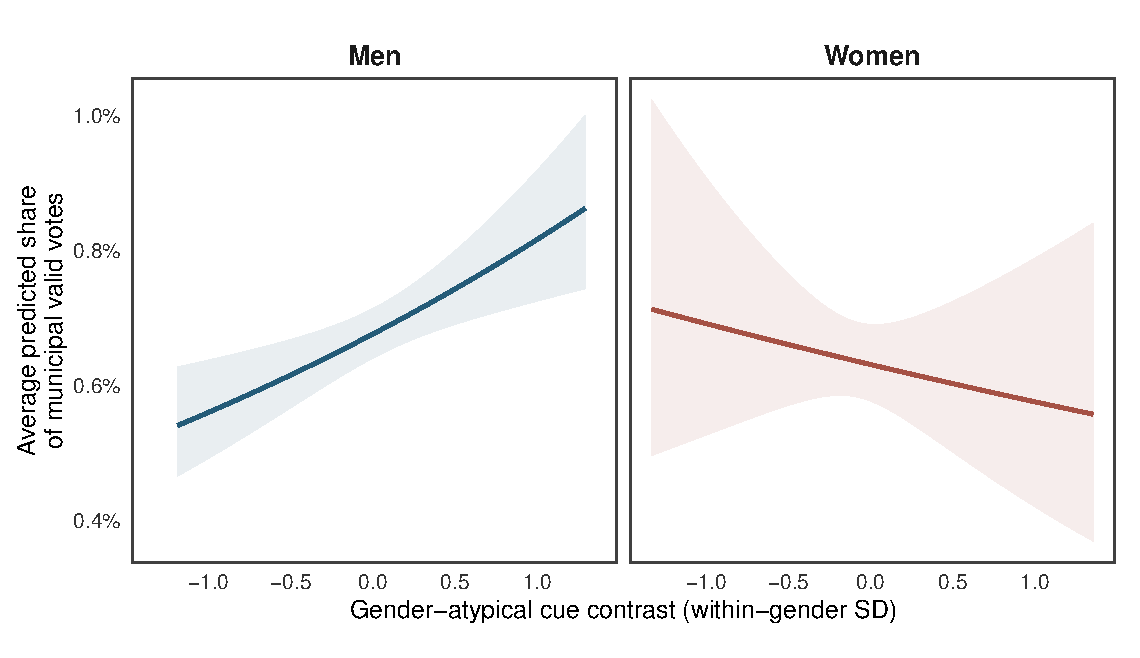
\includegraphics[width=0.92\linewidth]{figures/oa_baseline_predicted_vote_share.pdf}
\caption{Average predicted municipal vote share with baseline controls. Denominators include all valid personal votes in each municipality. Curves and municipality-clustered 95\% confidence intervals follow Figure~\ref{fig:predicted-votes}.}
\label{fig:predicted-share}
\end{figure}

\section{Baseline regression underlying the main results}
\label{sec:oa-baseline-regression}
Table~\ref{tab:oa-baseline-regression} reports the estimated coefficients of \autoref{eq:model}, the baseline Poisson model used to construct the predictions in Figure~\ref{fig:predicted-votes}. On the log conditional-mean scale, the male atypicality association is the coefficient on \texttt{Atypicality}, while the female association is its sum with the \texttt{Woman} $\times$ \texttt{Atypicality} coefficient. Table~\ref{tab:main} translates these associations into percentage differences in expected personal votes, whereas Figure~\ref{fig:predicted-votes} shows the resulting inequality in expected personal support across cue values.

\begin{table}[!htbp]
\centering\small
\caption{Baseline Poisson regression corresponding to Figure~\ref{fig:predicted-votes}}
\label{tab:oa-baseline-regression}
\begin{tabular}{@{}lrrcr@{}}
\toprule
Variable & Coefficient & Clustered SE & 95\% CI & $p$ \\
\midrule
\texttt{Atypicality} & 0.188 & 0.057 & [0.077, 0.300] & 0.001 \\
\texttt{Woman} & -0.312 & 0.125 & [-0.558, -0.066] & 0.013 \\
\texttt{Woman} $\times$ \texttt{Atypicality} & -0.280 & 0.145 & [-0.566, 0.005] & 0.054 \\
\texttt{Age} (mean centered) & 0.005 & 0.007 & [-0.008, 0.019] & 0.411 \\
\texttt{Attractiveness} & 1.048 & 0.140 & [0.771, 1.324] & $<0.001$ \\
\midrule
Municipality fixed effects & \multicolumn{4}{c}{Yes} \\
Party fixed effects & \multicolumn{4}{c}{Yes} \\
Candidates ($N$) & \multicolumn{4}{c}{1,384} \\
Municipalities ($G$) & \multicolumn{4}{c}{221} \\
\bottomrule
\end{tabular}
\par\smallskip
\begin{minipage}{\linewidth}\footnotesize
The dependent variable is personal votes. Coefficients and confidence intervals are on the log conditional-mean scale. Municipality-clustered standard errors (SE) incorporate a finite-sample correction. Confidence intervals (CI) and two-sided $p$-values use a $t$ reference distribution with 220 degrees of freedom. \texttt{Woman} indicates female candidates, with men as the reference category. Its coefficient compares genders at $A=0$. \texttt{Age} is centered at the sample mean of 45.76 years. \texttt{Attractiveness} enters in its original rating units. Municipality and party coefficients and the intercept are omitted from the table. The female atypicality association is the sum of the \texttt{Atypicality} and interaction coefficients. Its uncertainty uses their full covariance.
\end{minipage}
\end{table}

\FloatBarrier
\section{Party-specific contrasts and sensitivity analyses}
\label{sec:oa-party}
The baseline model pools the appearance-associated inequality across parties. The party-specific specification in \autoref{eq:party-model} allows the cue association and gender intercept to differ across parties. Table~\ref{tab:oa-party} reports the corresponding one-SD contrasts from the full municipality-clustered covariance matrix. Candidate and municipality counts describe the observations available within each party--gender cell. Inference uses the pooled model's 221 municipality clusters.

Because individual intervals do not test a common slope across parties, we also test whether the atypicality slopes are equal within each gender, using the full municipality-clustered covariance matrix. The joint test gives $F_{14,220}=10.07$ ($p<0.001$). The corresponding tests within men and women give $F_{7,220}=5.98$ ($p<0.001$) and $F_{7,220}=9.73$ ($p<0.001$), respectively. The joint test indicates that appearance-associated inequality varies across parties within one or both gender categories.

\begin{table}[!htbp]
\centering\small
\caption{Party-specific atypicality contrasts}
\label{tab:oa-party}
\begin{tabular}{llrrcr}
\toprule
Party & Gender & Candidates & Cell cities & Association (\%) & $p$ \\
\midrule
KD & Men & 134 & 66 & -19.6 [-41.2, 10.0] & 0.172 \\
KD & Women & 137 & 92 & 43.1 [-5.5, 116.9] & 0.090 \\
KESK & Men & 31 & 9 & -7.9 [-27.3, 16.7] & 0.493 \\
KESK & Women & 23 & 10 & 63.0 [30.8, 103.1] & $<0.001$ \\
KOK & Men & 59 & 17 & 22.1 [4.2, 43.1] & 0.014 \\
KOK & Women & 52 & 14 & -38.0 [-56.6, -11.4] & 0.009 \\
PS & Men & 357 & 154 & 19.1 [-5.6, 50.3] & 0.140 \\
PS & Women & 150 & 100 & -9.5 [-37.7, 31.4] & 0.598 \\
RKP & Men & 77 & 31 & 19.2 [-21.3, 80.7] & 0.405 \\
RKP & Women & 63 & 26 & -13.7 [-49.3, 46.8] & 0.585 \\
SDP & Men & 78 & 26 & 213.5 [84.9, 431.7] & $<0.001$ \\
SDP & Women & 63 & 27 & 0.4 [-27.6, 39.1] & 0.982 \\
VAS & Men & 53 & 17 & -3.1 [-21.3, 19.3] & 0.762 \\
VAS & Women & 49 & 18 & -26.1 [-42.8, -4.4] & 0.021 \\
VIHR & Men & 18 & 5 & 27.9 [11.5, 46.7] & $<0.001$ \\
VIHR & Women & 36 & 9 & -46.7 [-68.1, -11.2] & 0.016 \\
\bottomrule
\end{tabular}
\begin{minipage}{\linewidth}\footnotesize
Associations are percentage differences in expected personal votes for a one-SD increase in the cue contrast, with pointwise municipality-clustered 95\% intervals in brackets. The model uses 1380 candidates in 8 parties. Cell cities count municipalities represented in each gender--party group. Party codes correspond to the names in Figure~\ref{fig:party-votes}.
\end{minipage}
\end{table}

A joint difference across parties can coexist with sensitivity in any one party's estimated magnitude. Table~\ref{tab:oa-party-sensitivity} therefore examines whether party heterogeneity and the male contrasts discussed in the main text depend on prior political office or candidates with unusually many votes. Panel A reports the heterogeneity tests. Panel B compares the Social Democratic, National Coalition, and Green male contrasts. The office adjustment adds incumbent-councillor and national-MP indicators. The upper-tail exclusion uses the vote cutoff from the 99th percentile of the primary sample. Both retain the eligible party set and the primary sample's within-gender atypicality scaling. Party heterogeneity persists under both adjustments, although individual contrasts change in magnitude.

\begin{table}[!htbp]
\centering\footnotesize
\setlength{\tabcolsep}{3pt}
\caption{Sensitivity of the party-specific specification}
\label{tab:oa-party-sensitivity}
\textit{Panel A. Party heterogeneity tests}\par\smallskip
\begin{tabular}{p{0.32\linewidth}rrccc}
\toprule
Specification & $N$ & Cities & Joint $p$ & Men $p$ & Women $p$ \\
\midrule
Party-specific baseline & 1380 & 221 & $<0.001$ & $<0.001$ & $<0.001$ \\
+ Incumbency and parliamentary office & 1380 & 221 & $<0.001$ & 0.006 & $<0.001$ \\
Excluding top 1\% of votes & 1366 & 221 & $<0.001$ & $<0.001$ & $<0.001$ \\
\bottomrule
\end{tabular}\par\medskip\textit{Panel B. Selected male contrasts (\%)}\par\smallskip
\begin{tabular}{p{0.25\linewidth}p{0.22\linewidth}p{0.22\linewidth}p{0.22\linewidth}}
\toprule
Specification & Social Democrats & National Coalition & Green League \\
\midrule
Party-specific baseline & 213.5 [84.9, 431.7] & 22.1 [4.2, 43.1] & 27.9 [11.5, 46.7] \\
+ Incumbency and parliamentary office & 28.9 [-8.6, 81.7] & -4.9 [-18.4, 10.8] & 24.6 [7.7, 44.1] \\
Excluding top 1\% of votes & 79.8 [18.3, 173.1] & 23.0 [0.5, 50.7] & -27.7 [-40.8, -11.6] \\
\bottomrule
\end{tabular}
\begin{minipage}{\linewidth}\footnotesize
Heterogeneity tests use the full municipality-clustered covariance and test equal cue slopes across parties within gender. Each model includes $N$ candidates in $G$ municipality clusters. Panel B entries are percentage differences in expected votes with 95\% intervals. Adjustments do not identify a causal appearance effect.
\end{minipage}
\end{table}

\FloatBarrier
\section{Sensitivity analyses}
\label{sec:oa-sensitivity}
The pooled inequality may also depend on the comparison setting, target sample, and restrictions on control coefficients. Table~\ref{tab:oa-sensitivity} varies these features. Municipality-by-party fixed effects restrict comparisons to candidates on the same local party list. Singleton lists consequently do not identify cue slopes. To assess dependence on candidates with unusually many votes, upper-tail exclusions remove 14 candidates above the 99th percentile and 70 above the 95th percentile. These exclusions change the candidate population represented by the estimate. Finally, separate-gender models allow all coefficients, including the control associations, to differ between men and women.

\begin{table}[!htbp]
\centering
\caption{Atypical cue contrast under alternative adjustments}
\label{tab:oa-sensitivity}
\small\setlength{\tabcolsep}{3pt}
\begin{tabular}{p{0.32\linewidth}rrcc}
\toprule
Specification & $N$ & Cities & Men (\%) & Women (\%) \\
\midrule
Baseline controls & 1384 & 221 & 20.7 [8.0, 35.0] & -8.8 [-31.1, 20.8] \\
+ Joint cue level & 1384 & 221 & 20.4 [7.9, 34.4] & -13.5 [-37.7, 20.3] \\
+ Incumbency and parliamentary office & 1384 & 221 & 0.6 [-7.2, 9.1] & -10.7 [-26.2, 8.1] \\
Municipality-by-party fixed effects & 1211 & 160 & 31.4 [13.2, 52.6] & -8.8 [-40.0, 38.4] \\
Excluding top 1\% of votes & 1370 & 221 & 9.1 [-2.3, 21.8] & -7.0 [-21.9, 10.7] \\
Excluding top 5\% of votes & 1314 & 221 & -4.8 [-11.5, 2.3] & -7.0 [-15.9, 2.8] \\
Separate model for men & 810 & 191 & 20.2 [6.0, 36.3] & -- \\
Separate model for women & 574 & 178 & -- & -7.0 [-29.9, 23.4] \\
\bottomrule
\end{tabular}
\begin{minipage}{\linewidth}\footnotesize
Entries are percentage differences in expected votes for a one-SD increase in the atypical cue contrast, with municipality-clustered 95\% confidence intervals. Each model includes $N$ candidates in $G$ municipalities.
\end{minipage}
\end{table}

\FloatBarrier
\section{Political-experience adjustment}
Political experience provides a further reason candidates may attract different numbers of votes even conditional on age, appearance ratings, party, and municipality. We therefore add indicators for incumbent municipal councillors and members of the national parliament, referring to office held before the election. Holding the sample and baseline controls fixed, the expanded specification adds
\begin{equation}
 \log\mu_i^{\mathrm{office}}=\log\mu_i^{\mathrm{baseline}}
 +\rho_1\texttt{IncumbentCouncillor}_i+\rho_2\texttt{NationalMP}_i.
 \label{eq:office}
\end{equation}
The baseline linear predictor $\log\mu_i^{\mathrm{baseline}}$ follows \autoref{eq:model}, with all coefficients re-estimated in the expanded specification. The resulting one-SD atypicality associations are 0.6\% (95\% CI -7.2\% to 9.1\%) for men and -10.7\% (95\% CI -26.2\% to 8.1\%) for women. Figures~\ref{fig:oa-votes} and~\ref{fig:oa-share} express these associations as expected votes and municipal vote shares alongside the baseline predictions. Both specifications average over the same observed candidate contexts. The male appearance association is inconclusive after prior-office adjustment. Evidence for the baseline gradient is sensitive to this conditioning choice. Its point estimate lies closer to zero than in the baseline model.

\begin{figure}[!htbp]
\centering
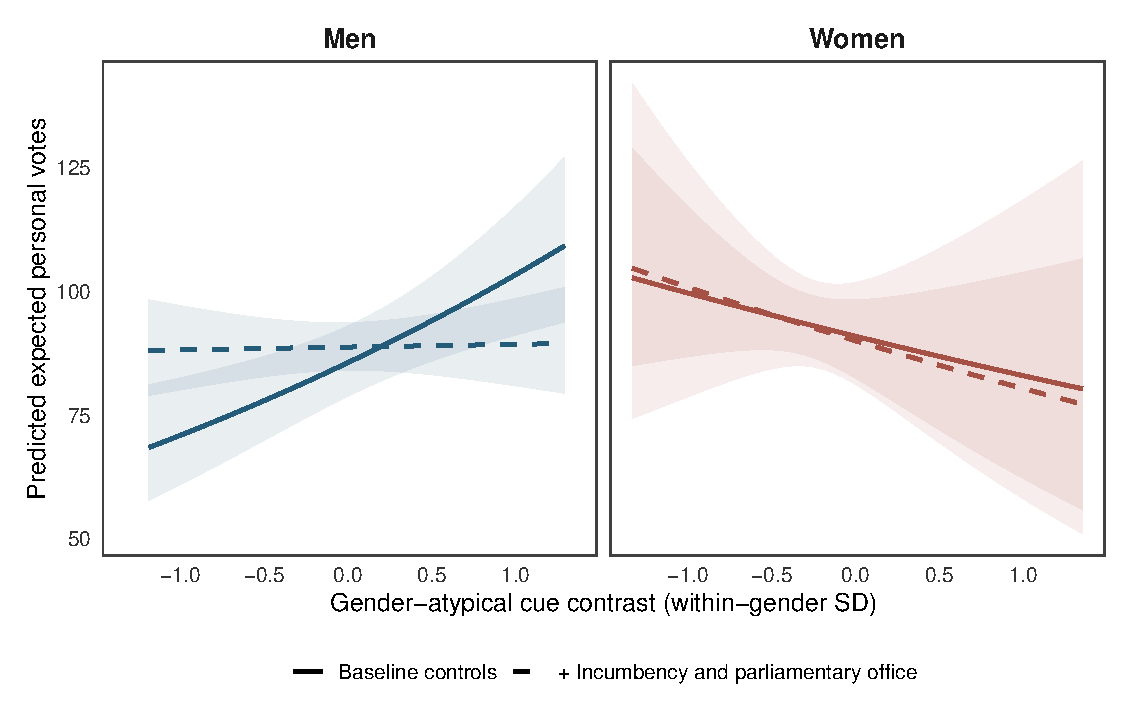
\includegraphics[width=0.92\linewidth]{figures/oa_predicted_votes.pdf}
\caption{Predicted expected personal votes with and without incumbency and parliamentary-office controls. Predictions are standardized over the same gender-specific observed candidate contexts. Shading denotes municipality-clustered 95\% confidence intervals.}
\label{fig:oa-votes}
\end{figure}

\begin{figure}[!htbp]
\centering
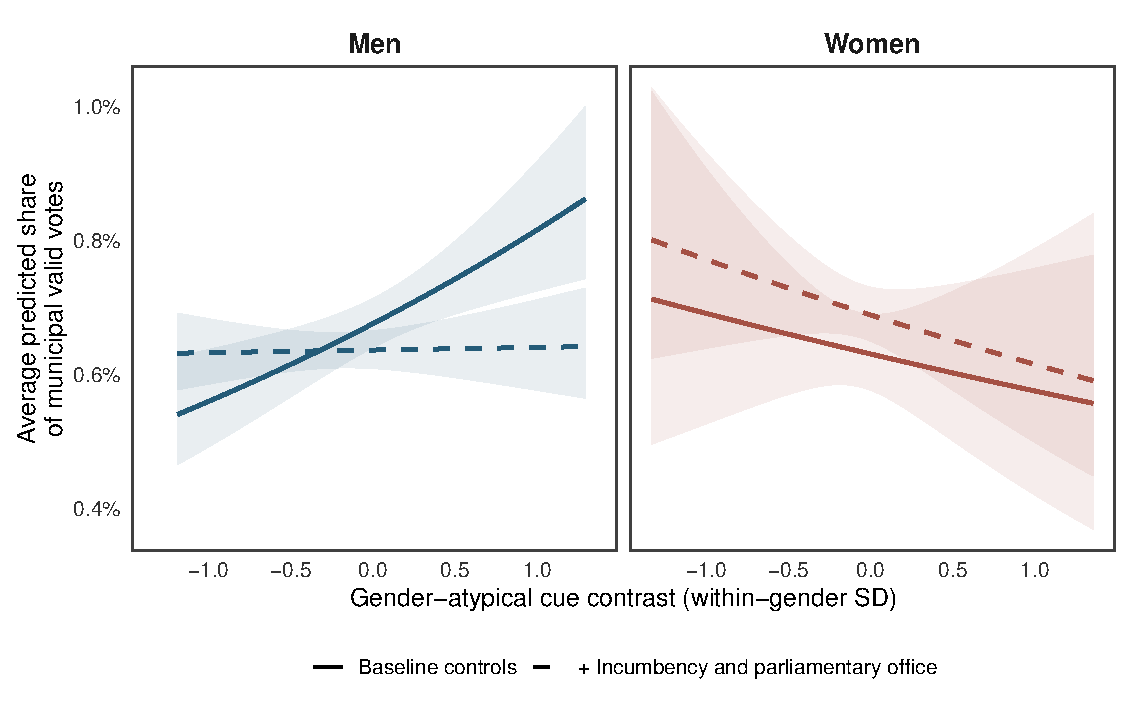
\includegraphics[width=0.92\linewidth]{figures/oa_predicted_vote_probability.pdf}
\caption{Average predicted municipal vote share with and without incumbency and parliamentary-office controls. Denominators include all valid personal votes in each municipality. Predictions and confidence intervals follow Figure~\ref{fig:oa-votes}.}
\label{fig:oa-share}
\end{figure}
\end{document}
